\documentclass[aspectratio=169]{beamer}

\usefonttheme[stillsansserifmath]{serif}
\usepackage{graphicx}
\usepackage{amsfonts}
\usepackage{mathtools, nccmath}
\usepackage{amssymb, amsmath}
\usepackage{xspace}
\usepackage{tikz}
\usepackage{standalone}
\usepackage{euler}
\usepackage{color,xcolor}
\usepackage{fontspec}
\usepackage{nameref}
\usepackage{manfnt}
\usepackage{listings}
\usepackage{xcolor}
\usepackage{algorithm}
\usepackage[noend]{algpseudocode}
\usepackage{algorithmicx}
\usepackage{docs/style}

\usepackage{xepersian}
\settextfont{Yas}

% Persian specific
\newcommand{\itmsep}[1]{\raggedleft\setlength\itemsep{#1}}
\newcommand{\itemr}{\raggedleft\setlength\itemsep{3mm}}
\newcommand{\fn}[2]{\LR{\LTRfootnote[frame,#1]{~#2}}}
%\newcommand{\fn}[2]{{\LR{\footnote[frame,#1]{{~\LR{#2}}}}}}
\newcommand{\fnn}[1]{{\LR{\footnote[frame]{{~\LR{#1}}}}}}
\newcommand{\m}[1]{\ensuremath{\mathnormal{#1}}}
\newcommand{\mc}[1]{\ensuremath{\mathtt{#1}}}
\newcommand{\scl}{\ensuremath{\Sigma^*}\xspace}
\newcommand{\gcl}{\ensuremath{\Gamma^*}\xspace}
\newcommand{\gin}{\ensuremath{\mathnormal{\in}}\xspace}
%\newcommand{\gand}{\ensuremath{\mathnormal{\land}}\xspace}
\newcommand{\gand}{\&\&\xspace}
\newcommand{\alglr}{\LTR\ttfamily\small}
\newcommand{\st}[1]{\ensuremath{\mathnormal{\{#1\}}}\xspace}
\newcommand{\gst}[1]{\ensuremath{\mathnormal{\{\text{\texttt{#1}}\}}}\xspace}
\newcommand{\cpp}{C++\xspace}
\newcommand{\enc}[1]{\ensuremath{\mathnormal{\langle#1\rangle}}\xspace}
\newcommand{\abo}[1]{\ensuremath{\mathnormal{O(#1)}}\xspace}
\newcommand{\aso}[1]{\ensuremath{\mathnormal{o(#1)}}\xspace}
\newcommand{\aom}[1]{\ensuremath{\mathnormal{\Omega(#1)}}\xspace}
\newcommand{\ath}[1]{\ensuremath{\mathnormal{\Theta(#1)}}\xspace}
\newcommand{\dom}[2]{\ensuremath{\mathnormal{\Big[ \dfrac{#1}{#2} \Big]}}\xspace}

\newcommand{\Proc}[2]{\Statex \textbf{procedure} \textsc{#1}(#2)}
\newcommand{\Func}[2]{\Statex \textbf{function} \textsc{#1}(#2)}
\newcommand{\To}{\textbf{to}\xspace}
\newcommand{\Aand}{\textbf{and}\xspace}
\newcommand{\Aor}{\textbf{or}\xspace}



\newcommand\pro{\ensuremath{\rightarrow}\xspace}
\newcommand\der{\ensuremath{\Rightarrow}\xspace}
\newcommand\ders{\ensuremath{\stackrel{\mbox{*}}{\Rightarrow}}\xspace}
\newcommand{\dern}[1]{\ensuremath{\stackrel{\mbox{\small #1}}{\Rightarrow}}\xspace}
\newcommand\move{\ensuremath{\vdash}\xspace}
\newcommand\moves{\ensuremath{\stackrel{\small *}{\vdash}}\xspace}
\newcommand{\movesn}[1]{\ensuremath{\stackrel{\small *}{\vdash_{#1}}}\xspace}
\newcommand{\moven}[1]{\ensuremath{\mathnormal{\vdash_{#1}}}\xspace}

\newcommand{\code}[1]{{\LR{\texttt{#1}}}}
\newcommand{\txtlr}[1]{\text{\LR{#1}}}


% Abbreviations
\newcommand{\ie}{\latin{i.e.,~}}
\newcommand{\eg}{\latin{e.g.,~}}
\newcommand{\cf}{\latin{cf.~}}
\newcommand{\etal}{\latin{et al.~}}
\newcommand{\etc}{\unskip~\latin{etc.}\xspace}
\newcommand{\apriori}{\latin{a priori}}
\newcommand{\wrt}{\latin{w.r.t.~}}
%\newtheorem{theorem}{Theorem}

\newcommand\NN{\ensuremath{\mathbb{N}}\xspace}
\newcommand\RR{\ensuremath{\mathbb{R}}\xspace}
\newcommand\NNS{\ensuremath{\mathbb{N}^*}\xspace}
\newcommand\NNZ{\ensuremath{\mathbb{N}\backslash\{0\}}\xspace}
\newcommand\RRP{\ensuremath{\mathbb{R}^+}\xspace}
\newcommand\vect[1]{\ensuremath{\boldsymbol{\vec{#1}}}}
\newcommand\MP{\ensuremath{\mathcal{P}}\xspace}

\newcommand\de{\mathrel{\bullet\mkern-2.5mu{\rightarrow}}}
\newcommand\ue{\mathrel{\bullet\mkern-3mu{-}\mkern-3mu\bullet}}

\DeclareMathOperator*{\argmax}{arg\,max}
\DeclareMathOperator*{\argmin}{arg\,min}

\DeclareMathOperator{\lcm}{lcm}
\DeclareMathOperator{\Spec}{Spec}
\DeclareMathOperator{\Res}{Res}
%\DeclareMathOperator{\land}{and}

\newcommand{\fl}[1]{\ensuremath{\lfloor #1 \rfloor}}
\newcommand{\bfl}[1]{\ensuremath{\big\lfloor #1 \big\rfloor}}
\newcommand{\Bfl}[1]{\ensuremath{\Big\lfloor #1 \Big\rfloor}}
\newcommand{\bgfl}[1]{\ensuremath{\bigg\lfloor #1 \bigg\rfloor}}
\newcommand{\Bgfl}[1]{\ensuremath{\Bigg\lfloor #1 \Bigg\rfloor}}

\newcommand{\cl}[1]{\ensuremath{\lceil #1 \rceil}}
\newcommand{\bcl}[1]{\ensuremath{\big\lceil #1 \big\rceil}}
\newcommand{\Bcl}[1]{\ensuremath{\Big\lceil #1 \Big\rceil}}
\newcommand{\bgcl}[1]{\ensuremath{\bigg\lceil #1 \bigg\rceil}}
\newcommand{\Bgcl}[1]{\ensuremath{\Bigg\lceil #1 \Bigg\rceil}}

\newcommand{\mtx}[1]{\begin{pmatrix} #1 \end{pmatrix}}
\newcommand{\smtx}[1]{\begin{psmallmatrix} #1 \end{psmallmatrix}}

\definecolor{commentgreen}{RGB}{2,112,10}
\definecolor{eminence}{RGB}{108,48,130}
\definecolor{brightmaroon}{rgb}{0.76, 0.13, 0.28}
\definecolor{darkred}{rgb}{0.55, 0.0, 0.0}
\lstset {
    language=C++,
    frame=tb,
    tabsize=4,
    showstringspaces=false,
    numbers=left,
    %upquote=true,
    commentstyle=\color{commentgreen},
    keywordstyle=\color{eminence},
    stringstyle=\color{darkred},
    basicstyle=\small\ttfamily, % basic font setting
    emph={int,char,double,float,unsigned,long,short,void,bool},
    emphstyle={\color{blue}},
    %escapechar=\&,
    % keyword highlighting
    %classoffset=1, % starting new class
    %otherkeywords={>,<,.,;,-,!,=,~},
    %morekeywords={>,<,.,;,-,!,=,~},
    %keywordstyle=\color{weborange},
    %classoffset=0,
}

\makeatletter
\NewDocumentCommand{\LeftComment}{s m}{%
	\IfBooleanF{#1}{\hspace*{\ALG@thistlm}}\textcolor{commentgreen}{\(~\triangleright\) #2}}
\makeatother


\newenvironment{itemframe}[2]{
\begin{frame}[environment=itemframe]{#1}

\framesubtitle{\small \color{gray} \quad #2}
\itemize
\itemr

}{
\enditemize
\end{frame}
}

\newcommand{\centerimg}[2][.5]{
    \begin{figure}[h!]
        \centering
        \includegraphics[width=#1\textwidth]{#2}
    \end{figure}
}

\usetikzlibrary{arrows,calc}
\usetikzlibrary{positioning,shapes,chains,fit}


\tikzset{
    %Define style for boxes
    node/.style={
        circle,
        draw=black, thick,
        align=center,
    },
    ss/.style={
        circle,
        draw=black,
        align=center,
    },
    proc/.style={
        rounded corners,
        draw=black,
        align=center,
    },
    ifelse/.style={
	ellipse,
	draw=black,
	align=center,
    },
    cloudy/.style={
	cloud,
	cloud puffs=12,
	cloud ignores aspect,
	align=center,
	draw=black,
    },
    txt/.style={
        draw = none,
        align = center,
        font = \footnotesize,
    },
    coin/.style={
        rectangle,
        minimum height=1mm,
        minimum width=1cm,
        draw=black,
        fill=black!20,
        rounded corners
    },
    towercolor/.style={
        fill=black!80
    },
    towerbase/.style={
        trapezium,
        trapezium angle=75,
        trapezium stretches=true,
        towercolor,
        minimum width=7mm,
        minimum height=2mm,
    },
    tower/.style={
        rectangle,
        rounded corners,
        towercolor,
        minimum width=2mm,
        minimum height=26mm,
    },
    start-end/.style={
        draw,
        rectangle,
        rounded corners,
    },
    input/.style={ % requires library shapes.geometric
        draw,
        trapezium,
        trapezium left angle=60,
        trapezium right angle=120,
    },
    operation/.style={
        draw,
        rectangle
    },
    loop/.style={ % requires library shapes.misc
        draw,
        chamfered rectangle,
        chamfered rectangle xsep=2cm
    },
    decision/.style={ % requires library shapes.geometric
        draw,
        diamond,
        aspect=#1
    },
    decision/.default=1,
    print/.style={ % requires library shapes.symbols
        draw,
        tape,
        tape bend top=none
    },
    connection/.style={
        draw,
        circle,
        radius=5pt,
    },
    process rectangle outer width/.initial=0.15cm,
    predefined process/.style={
        rectangle,
        draw,
        append after command={
        \pgfextra{
          \draw
          ($(\tikzlastnode.north west)-(0,0.5\pgflinewidth)$)--
          ($(\tikzlastnode.north west)-(\pgfkeysvalueof{/tikz/process rectangle outer width},0.5\pgflinewidth)$)--
          ($(\tikzlastnode.south west)+(-\pgfkeysvalueof{/tikz/process rectangle outer width},+0.5\pgflinewidth)$)--
          ($(\tikzlastnode.south west)+(0,0.5\pgflinewidth)$);
          \draw
          ($(\tikzlastnode.north east)-(0,0.5\pgflinewidth)$)--
          ($(\tikzlastnode.north east)+(\pgfkeysvalueof{/tikz/process rectangle outer width},-0.5\pgflinewidth)$)--
          ($(\tikzlastnode.south east)+(\pgfkeysvalueof{/tikz/process rectangle outer width},0.5\pgflinewidth)$)--
          ($(\tikzlastnode.south east)+(0,0.5\pgflinewidth)$);
        }  
        },
        text width=#1,
        align=center
    },
    predefined process/.default=1.75cm,
    man op/.style={ % requires library shapes.geometric
        draw,
        trapezium,
        shape border rotate=180,
        text width=2cm,
        align=center,
    },
    extract/.style={
        draw,
        isosceles triangle,
        isosceles triangle apex angle=60,
        shape border rotate=90
    },
    merge/.style={
        draw,
        isosceles triangle,
        isosceles triangle apex angle=60,
        shape border rotate=-90
    },
}


\title{طراحی الگوریتم‌ها}
\author{
آرش شفیعی
}

\institute{
\\

\includegraphics[height=1.2cm]{logos/ui.png}
%\\
%دانشگاه اصفهان
}
\date{}

\begin{document}

\begin{frame}[plain]
\begin{center}
به نام خدا
\end{center}

\maketitle

%\begin{center}
%{\footnotesize arash.shafiei@gmail.com}
%\end{center}

\end{frame}
\setcounter{framenumber}{0}

%\input{docs/licence}

\raggedleft

%%%%%%%%%%%%
%\begin{frame}{فهرست مطالب}
%\begin{flushright}
%  \tableofcontents
%\end{flushright}
%\end{frame}
%%%%%%%%%%%%

%%%%%%%%%%%%
\begin{itemframe}{مقدمه}
\itm
بسیاری از مسائل محاسباتی کاربردی ان‌پی کامل هستند و با این حال با توجه به اهمیت زیادی که دارند نیاز داریم جوابی برای آنها پیدا کنیم گرچه پیدا کردن جواب دقیق برای اینگونه مسائل در زمان چندجمله‌ای امکان‌پذیر نیست.
\itm
وقتی یک مسئله ان‌پی کامل است، برای حل آن سه راه پیش رو داریم : (۱) اگر ورودی نسبتاً کوچک باشد، می‌توان یک جواب بهینه در زمان نمایی به سرعت برای آن پیدا کرد. (۲) می‌توان یک حالت خاص از مسئله را در زمان چند جمله‌ای حل کرد. (۳) می‌توان یک جواب نزدیک به جواب بهینه در زمان چند جمله‌ای برای آن پیدا کرد. در بسیاری از کاربردها جواب نزدیک به جواب بهینه
\fn{near-optimal solution}
نیز کافی است. به چنین الگوریتم‌هایی که جواب نزدیک به بهینه تولید می‌کنند، الگوریتم‌های تقریبی
\fn{approximation algorithm}
می‌گوییم. برای بسیاری از مسائل ان‌پی کامل می‌توان یک الگوریتم تقریبی در زمان چندجمله‌ای پیدا کرد.
\end{itemframe}


\begin{itemframe}{مقدمه}
\itm
فرض کنید بر روی مسئلهٔ بهینه‌سازی کار می‌کنید که در آن هر یک از جواب‌های بالقوه
\fn{potential solution}
دارای یک هزینه است و می‌خواهید یک جواب نزدیک به بهینه پیدا کنید. بسته به نوع مسئله، ممکن است مسئله بیشینه سازی
\fn{maximization}
یا کمینه سازی
\fn{minimization}
باشد. می‌توانید یک جواب بهینه با هزینه حداکثر یا هزینه حداقل پیدا کنید.
\end{itemframe}

\begin{itemframe}{مقدمه}
\itm
می‌گوییم یک الگوریتم دارای «ضرب تقریب»
\fn{approximation ratio}
$\rho(n)$
است اگر به ازای هر ورودی با اندازهٔ n ، هزینهٔ
$C$
جواب تولید شده توسط الگوریتم نسبت به هزینهٔ
$C^*$
مربوط به جواب بهینه از مقدار
$\rho(n)$
کمتر باشد. به عبارت دیگر :
$$
\Bigl\{ \frac{C}{C^*}, \frac{C^*}{C} \Bigr\} \leqslant \rho(n)
$$
\itm
اگر یک الگوریتم دارای ضریب تقریب
$\rho(n)$
باشد، به آن الگوریتم تقریبی
$\rho(n)$
می‌گوییم.
\end{itemframe}


\begin{itemframe}{مقدمه}
\itm
از الگوریتم‌های تقریبی
$\rho(n)$
هم برای مسائل کمینه سازی و هم برای مسائل بیشینه سازی استفاده می‌شود.
\itm
در یک مسئله بیشینه سازی، داریم
$0 < C \leqslant C^*$
و بنابراین مقدار
$C^*/C$
مقدار بزرگ‌تری است که در آن هزینهٔ جواب بهینه از هزینهٔ جواب تقریبی بزرگ‌تر است.
\itm
در یک مسئله کمینه سازی، داریم
$0 < C^* \leqslant C$
و بنابراین مقدار
$C/C^*$
مقدار بزرگ‌تری است که در آن هزینهٔ جواب تقریبی از هزینهٔ جواب بهینه بزرگ‌تر است.
\itm
با فرض اینکه همهٔ هزینه‌ها مقادیر مثبت هستند، ضریب تقریب در یک الگوریتم تقریبی هیچ‌گاه کمتر از ۱ نیست.
\iffalse
 زیرا اگر داشته باشیم
$C/C^* \leqslant 1$
آنگاه
$C^*/C \geqslant 1$
.
\fi
\itm
بنابراین یک الگوریتم تقریبی با ضریب ۱ جوابی بهینه تولید می‌کند و هر چه ضریب تقریب الگوریتم تقریبی بیشتر باشد، جواب به دست آمده از جواب بهینه دورتر است.
\end{itemframe}


\begin{itemframe}{مقدمه}
\itm
برای بسیاری از مسائل، الگوریتم‌های تقریبی چند جمله‌ای با ضریب تقریب کوچک وجود دارد و برای برخی دیگر از مسائل، الگوریتم‌های تقریبی دارای ضریب تقریبی هستند که با مقدار n افزایش پیدا می‌کند.
\itm
در برخی از الگوریتم‌های تقریبی چندجمله‌ای، هرچه الگوریتم در زمان بیشتری اجرا شود، ضریب تقریب بهتری به دست می‌آید. در چنین مسائلی می‌توان با افزایش زمان محاسبات ضریب تقریب را بهبود داد.
\itm
این وضعیت حائز اهمّیت است و یک ناگذاری برای آن وجود دارد که در ادامه معرفی می‌کنیم.
\end{itemframe}

%todo this part is only usefull if an example of Approximation Scheme is mentioned delete it otherwise
\begin{itemframe}{مقدمه}
\itm
طرح تقریب
\fn{Approximation Scheme}
برای یک مسئلهٔ بهینه‌سازی، الگوریتمی تقریبی است که یک نمونه از مسئله را همراه با مقدار
$\varepsilon > 0$
دریافت می‌کند، به طوری که این الگوریتم یک الگوریتم تقریبی
$(1 + \varepsilon)$
 باشد.
\itm
اگر این طرح تقریب برای هر مقدار
$\epsilon > 0$
در زمانی چندجمله‌ای نسبت به اندازهٔ ورودی $n$ اجرا شود، آن را طرح تقریب چندجمله‌ای
\fn{Polynomial-Time Approximation Scheme}
 می‌نامیم.
\itm
زمان اجرای یک طرح تقریب چند جمله‌ایی ممکن است با کاهش
$\epsilon$
 به شدت افزایش یابد. برای مثال زمان اجرای آن می‌تواند چنین چیزی باشد:
$$
O(n^{2/\epsilon})
$$
\end{itemframe}


\begin{itemframe}{مقدمه}
\itm
اگر یک طرح تقریب، زمان اجرای چندجمله‌ای نسبت به هر دو پارامتر
$1/\varepsilon$
و $n$ داشته‌باشد، آن را «طرح تقریب چندجمله‌ای کامل»

\fn{Fully Polynomial-Time Approximation Scheme}
می‌نامیم. زمان اجرای یک طرح تقریب چند جمله‌ایی کامل می‌تواند چنین باشد:
$$
O((1/\epsilon)^2n^3)
$$
\itm
در چنین الگوریتمی، هر کاهش با ضریب ثابت در $\epsilon$، باعث افزایش زمان اجرا به‌اندازهٔ یک ضریب ثابت می‌شود.
\end{itemframe}

\begin{frame}{‌ضرب زنجیره‌ای ماتریس‌ها}
\begin{itemize}\itemr
\item[-]
مسئلهٔ ضرب زنجیره‌ای ماتریس‌ها
\fn{1}{Matrix-chain multiplication problem}
 به صورت زیر است. می‌خواهیم دنباله (زنجیره)ای از n ماتریس
\m{\langle A_1, A_2, \cdots, A_n \rangle}
را در هم ضرب کنیم. این ماتریس‌ها الزاماً ماتریس‌های مربعی نیستند و هدف این است که در این ضرب ماتریسی کمترین تعداد عملیات ضرب استفاده شود.
\item[-]
ضرب ماتریس‌ها شرکت پذیر
\fn{2}{associative}
، بدین معنی که پرانتز گذاری به هر نحوی انجام می‌شود، جواب ضرب ماتریسی تغییر نخواهد کرد.
\end{itemize}
\end{frame}


\begin{frame}{‌ضرب زنجیره‌ای ماتریس‌ها}
\begin{itemize}\itemr
\item[-]
الگوریتم ضرب دو ماتریس
\m{A(a_{ij})}
و
\m{B(b_{ij})}
به صورت زیر است. نتیجه ضرب این دو ماتریس در ماتریس
\m{C(c_{ij})}
ذخیره می‌شود.
\begin{algorithm}[H]\alglr
  \caption{Matrix Multiplication} 
  \begin{algorithmic}[1]
   \Func{Rectangular-Matrix-Multiply}{A, B, C, p, q, r}
     \For{i = 1 to p}
     	\For{j = 1 to r}
     		\For{k = 1 to q}
      			\State c[i,j] += a[i,k] * b[k,j]
     		\EndFor
     	\EndFor     		      			
     \EndFor                            
  \end{algorithmic}
  \label{alg:merge}
\end{algorithm}
\item[-]
برای اینکه ضرب ماتریسی درست باشد لازم است ابعاد ماتریس A برابر با
\m{p \times q}
و ابعاد ماتریس B برابر با
\m{q \times r}
باشد و ابعاد ماتریس حاصلضرب C در اینصورت برابر با
\m{p \times r}
خواهد بود. تعداد عملیات ضرب انجام شده برابر است با
\m{pqr}.
\end{itemize}
\end{frame}


\begin{frame}{‌ضرب زنجیره‌ای ماتریس‌ها}
\begin{itemize}\itemr
\item[-]
زنجیره ضرب ماتریسی
\m{A_1 \cdot A_2 \cdot A_3}
را در نظر بگیرید. فرض کنید ماتریس
\m{A_1}
با ابعاد
\m{10 \times 100}
، ماتریس
\m{A_2}
با ابعاد
\m{100 \times 5}
و ماتریس
\m{A_3}
با ابعاد
\m{5 \times 50}
باشد. اگر پرانتز گذاری به صورت
\m{((A_1A_2)A_3)}
باشد، تعداد
\m{10 \times 100 \times 5 = 5000}
عملیات ضرب برای ضرب
\m{A_1A_2}
و تعداد
\m{10 \times 5 \times 50 = 2500}
عملیات ضرب برای ضرب
\m{A_3}
در حاصلضرب
\m{A_1A_2}
باید انجام شود. بنابراین نیاز به انجام
\m{7500}
عملیات ضرب است.
\item[-]
حال فرض کنید پرانتز گذاری به صورت
\m{(A_1(A_2A_3))}
باشد. در اینصورت نیاز به انجام
\m{100 \times 5 \times 50 = 25000}
عملیات ضرب برای ضرب
\m{A_2A_3}
و نیاز به انجام 
\m{10 \times 100 \times 50 = 50000}
عملیات ضرب
برای ضرب
\m{A_1}
در حاصلضرب 
\m{A_2 A_3}
است،
بنابراین در مجموع نیاز به انجام
\m{75000}
عملیات ضرب است. بنابراین با استفاده از پرانتز گذاری اول، عملیات ضرب ۱۰ برابر سریع‌تر انجام می‌شود.
\end{itemize}
\end{frame}


\begin{frame}{‌ضرب زنجیره‌ای ماتریس‌ها}
\begin{itemize}\itemr
\item[-]
مسئله ضرب زنجیره‌ای ماتریس‌ها
را به صورت زیر بیان می‌کنیم :\\
زنجیرهٔ n ماتریس
\m{\langle A_1, A_2, \cdots, A_n \rangle}
را در نظر بگیرید، به طوری‌که به ازای
\m{i = 1,2, \cdots , n}
، ابعاد ماتریس
\m{A_i}
برابر است با
\m{p_{i-1} \times p_i}
. ضرب
\m{A_1 \cdot A_2 \cdots A_n}
را طوری پرانتز گذاری کنید که تعداد ضرب‌ها در عملیات ضرب این زنجیرهٔ ماتریسی حداقل باشد. ابعاد ورودی مسئله به صورت
\m{\langle p_0, p_1, p_2, \cdots, p_n \rangle}
داده شده‌اند.
\item[-]
در مسئله ضرب زنجیره‌ای ماتریس‌ها نمی‌خواهیم حاصلضرب ماتریس‌ها را به دست آوریم بلکه تنها می‌خواهیم ترتیب ضرب را به گونه‌ای به دست آوریم که هزینه ضرب به حداقل برسد. معمولا زمانی که صرف پیدا کردن پرانتز گذاری بهینه می‌شود ارزش هزینه کردن دارد، چرا که ممکن است ضرب ماتریس‌ها به صورت ترتیبی هزینهٔ گزافی به کاربر تحمیل کند.
\end{itemize}
\end{frame}


\begin{frame}{‌ضرب زنجیره‌ای ماتریس‌ها}
\begin{itemize}\itemr
\item[-]
قبل از اینکه این مسئله را حل کنیم، بررسی می‌کنیم چند پرانتز گذاری متفاوت وجود دارد. در واقع یک الگوریتم ساده برای حل این مسئله این است که هزینهٔ همهٔ پرانتز گذاری‌ها را با یکدیگر مقایسه کنیم ولی از آنجایی که تعداد پرانتز‌ گذاری‌ها بسیار زیاد است، بررسی همهٔ حالات مقدور نیست.
\item[-]
فرض کنید تعداد کل حالات برای پرانتز گذاری n ماتریس برابر باشد با
\m{P(n)}.
وقتی
\m{n = 1}
تنها یک ماتریس در زنجیره وجود دارد و بنابراین تنها یک حالت برای پرانتز گذاری وجود دارد. وقتی
\m{n \geqslant 2}
باشد، درواقع عبارت می‌تواند به دو قسمت شکسته شود به طوری‌که هر قسمت به طور جداگانه پرانتز گذاری شود. تعداد کل حالت‌های پرانتز گذاری برابر است با ضرب تعداد حالات پرانتز گذاری قسمت اول ضرب در تعداد حالت‌های پرانتز گذاری قسمت دوم.
\end{itemize}
\end{frame}


\begin{frame}{‌ضرب زنجیره‌ای ماتریس‌ها}
\begin{itemize}\itemr
\item[-]
این زنجیره می‌تواند به شکل‌های متعددی به دو قسمت تقسیم شود که با احتساب همهٔ حالت‌ها عبارت زیر را برای تعداد کل حالت‌های پرانتز گذاری به دست می‌آوریم.
\begin{align*}
\m{P(n)} = \left\{ \begin{array}{lr}
\m{1} & \m{n = 1}~~ \text{اگر}\\
\m{\sum_{k = 1}^{n - 1} P(k) P(n-k)} & \m{n \geqslant 2}~~ \text{اگر}
\end{array}\right.
\end{align*}
\item[-]
با حل این رابطهٔ بازگشتی به دست می‌آید
\m{P(n) = \Omega (2^n)}.
در واقع
\m{P(n)}
دنبالهٔ اعداد کاتالان
\fn{1}{catalan numbers}
(1, 1, 2, 5, 14, 42, 132, 429, 1430, 4862, 16796, 58786, ...)
را می‌سازد که رشد آن نمایی است و بنابراین به ازای n ‌های بسیار بزرگ، بررسی کردن همهٔ حالت‌ها در عمل غیرممکن است.
\end{itemize}
\end{frame}


\begin{frame}{‌ضرب زنجیره‌ای ماتریس‌ها}
\begin{itemize}\itemr
\item[-]
حال از روش برنامه‌ریزی پویا برای بهینه‌سازی پرانتز گذاری زنجیرهٔ ماتریسی استفاده می‌کنیم. یک الگوریتم به روش برنامه‌ریزی پویا برای یک مسئلهٔ بهینه‌سازی از چهار مرحله تشکیل شده است :
\item[۱-]
توصیف ساختار جواب بهینه بر اساس جواب بهینه زیرمسئله‌ها و بررسی اصل بهینگی
\item[۲-]
تعریف کردن مقدار جواب بهینه به طور بازگشتی
\item[۳-]
محاسبه کردن مقدار جواب بهینه
\item[۴-]
ساختن جواب بهینه توسط اطلاعات محاسبه شده
\end{itemize}
\end{frame}


\begin{frame}{‌ضرب زنجیره‌ای ماتریس‌ها}
\begin{itemize}\itemr
\item[-]
برای حل یک مسئلهٔ بهینه‌سازی توسط برنامه‌ریزی پویا باید مسئله دارای زیرساختار بهینه
\fn{1}{optimal substructure}
 باشد یا به عبارت دیگر اصل بهینگی
\fn{2}{principle of optimality}
  در آن برقرار باشد.
\item[-]
یک مسئله دارای زیرساختار بهینه است اگر جواب بهینه برای یک مسئله، شامل جواب‌های زیرمسئله‌ها باشد. به عبارت دیگر اگر جواب یک مسئلهٔ بهینه‌سازی را به دست آوریم، باید بتوانیم از جواب آن برای زیرمسئله‌ها نیز استفاده کنیم.
\item[-]
برای مثال مسئله کوتاهترین مسیر در گراف دارای زیرساختار بهینه است.
اگر کوتاهترین مسیر از x به y را به دست آوریم به طوری که مسیر از z عبور کند، کوتاهترین مسیر از x به z  و همچنین کوتاهترین مسیر از z به y نیز در جواب مسئله به دست آمده است.
\item[-]
اما مسئله بلندترین مسیر دارای زیرساختار بهینه نیست.
اگر بلندترین مسیر از x به y را به دست آوریم به طوری که مسیر از z عبور کند، نمی‌توانیم بگوییم بلندترین مسیر از z به y نیز در جواب مسئله است، زیرا ممکن است بلندترین مسیر از z به y از x عبور کند.
\end{itemize}
\end{frame}


\begin{frame}{‌ضرب زنجیره‌ای ماتریس‌ها}
\begin{itemize}\itemr
\item[-]
(گام ۱) توصیف ساختار جواب بهینه بر اساس جواب زیرمسئله‌ها و بررسی اصل بهینگی:
\item[-]
اولین مرحله در برنامه‌ریزی پویا تشخیص دادن ساختاری از مسئله است که در زیر مسئله‌ها نیز تکرار می‌شود. به عبارت دیگر اگر مسئله را برای یک زیر مسئله حل کنیم، باید بتوانیم با استفاده از اطلاعات زیر مسئله، مسئله را حل کنیم.
\item[-]
فرض کنید به ازای
\m{i \leqslant j}
ماتریس
\m{A_{i : j}}
از ضرب ماتریس‌های
\m{A_i A_{i+1} \cdots A_j}
به دست بیاید. اگر
\m{i = j}
باشد تنها یک پرانتز گذاری وجود دارد، اما اگر
\m{i < j}
باشد آنگاه برای پرانتز گذاری این عبارت می‌توانیم آن را به دو قسمت
\m{A_{i : k}}
و
\m{A_{k+1 : j}}
تقسیم کنیم به طوری‌که
\m{ i \leqslant k < j} .
با ضرب این دو ماتریس در یکدیگر، حاصل
\m{A_{i : j}}
را به دست می‌آوریم.
هزینهٔ پرانتز گذاری
\m{A_{i : j}}
برابر است با هزینه پرانتز گذاری
\m{A_{i : k}}
به علاوهٔ هزینهٔ پرانتز گذاری
\m{A_{k+1 : j}}
به علاوهٔ هزینهٔ ضرب دو قسمت در یکدیگر.
\end{itemize}
\end{frame}


\begin{frame}{‌ضرب زنجیره‌ای ماتریس‌ها}
\begin{itemize}\itemr
\item[-]
مسئلهٔ ضرب زنجیره‌ای ماتریس‌ها دارای زیرساختار بهینه است. به عبارت دیگر اگر یک پرانتزگذاری برای 
\m{A_{i:j}}
پیدا کنیم به طوری که به دو قسمت 
\m{A_{i:k}}
و
\m{A_{k+1:j}}
تقسیم شود، پرانتزگذاری
\m{A_{i:k}}
نیز بهینه است (به همین ترتیب پرانتزگذاری 
\m{A_{k+1:j}}
نیز بهینه است)
.
\item[-]
اثبات: فرض کنیم پرانتزگذاری 
\m{A_{i:j}}
 بهینه باشد و پرانتزگذاری
\m{A_{i:k}}
بهینه نباشد. در اینصورت می‌توانیم یک پرانتزگذاری بهینه برای 
\m{A_{i:k}}
پیدا کنیم و آن را در 
\m{A_{i:j}}
استفاده کنیم و یک پرانتزگذاری با هزینه کمتر برای 
\m{A_{i:j}}
به دست آوریم که با فرض اولیه در تناقض است. 
\end{itemize}
\end{frame}


\begin{frame}{‌ضرب زنجیره‌ای ماتریس‌ها}
\begin{itemize}\itemr
\item[-]
به طور خلاصه، اگر پرانتزگذاری بهینه برای
\m{A_{i : j}}
را پیدا کنیم، این پرانتزگذاری الزاما از دو پرانتزگذاری
\m{A_{i : k}}
و
\m{A_{k+1 : j}}
تشکیل شده است و الزاما پرانتزگذاری‌های
\m{A_{i : k}}
و
\m{A_{k+1 : j}}
نیز بهینه هستند.
\item[-]
بدین دلیل می‌توانیم از برنامه‌ریزی پویا استفاده کنیم، زیرا می‌توانیم هزینه‌های پرانتزگذاری‌های
\m{A_{i : k}}
و
\m{A_{k+1 : j}}
را از قبل ذخیره کنیم، و از این هزینه‌ها برای محاسبهٔ پرانتزگذاری
\m{A_{i : j}}
استفاده کنیم.
\end{itemize}
\end{frame}


\begin{frame}{‌ضرب زنجیره‌ای ماتریس‌ها}
\begin{itemize}\itemr
\item[-]
بنابراین باید مقدار 
\m{k}
 را پیدا کنیم به طوری‌که هزینهٔ پرانتز گذاری
\m{A_{i : k}}
به علاوهٔ هزینهٔ‌ پرانتزگذاری
\m{A_{k+1 : j}}
به علاوهٔ هزینهٔ ضرب
\m{A_{i : k}}
در
\m{A_{k+1 : j}}
بهینه باشد. آنگاه پرانتز گذاری
\m{A_{i : j}}
نیز بهینه خواهد بود.
\item[-]
پس برای حل مسئله یافتن هزینهٔ پرانتزگذاری بهینه برای
\m{A_{i : j}}
باید به ازای همهٔ 
\m{k}
 ها
هزینهٔ‌ پرانتزگذاری بهینه برای 
\m{A_{i : k}}
و 
\m{A_{k+1 : j}}
را محاسبه و با هزینهٔ ضرب
\m{A_{i : k}}
در
\m{A_{k+1 : j}}
جمع کنیم.
آنگاه از این میان 
\m{k}
 را به گونه‌ای انتخاب کنیم که هزینهٔ پرانتزگذاری 
بهینه باشد (تعداد ضرب‌های پرانتزگذاری
\m{A_{i : j}}
 کمترین مقدار ممکن باشد).
\iffalse
\item[-]
عبارت قبل را می‌توانیم به صورت زیر با استفاده از برهان خلف ثابت کنیم. فرض کنیم پرانتز گذاری
\m{A_{i : j}}
بهینه نباشد. این بدین معناست که یک پرانتز گذاری با هزینه کمتر وجود دارد. اما اگر یک پرانتز گذاری بهینه‌تر وجود داشته باشد می‌توان عبارت
\m{A_{i : j}}
را به دو قسمت تقسیم کرد و یک پرانتز گذاری بهتر برای
\m{A_{i : k}}
و
\m{A_{k+1 : j}}
پیدا کرد که در اینصورت به تناقض می‌رسیم.
\fi
\end{itemize}
\end{frame}



\begin{frame}{‌ضرب زنجیره‌ای ماتریس‌ها}
\begin{itemize}\itemr
\item[-]
(گام ۲) تعریف کردن مقدار جواب بهینه به طور بازگشتی :
\item[-]
فرض کنید
\m{m[i,j]}
حداقل تعداد ضرب‌های مورد نیاز برای محاسبه
\m{A_{i : j}}
باشد. حداقل تعداد ضرب‌های مورد نیاز برای کل n ماتریس یعنی
\m{A_{1 : n}}
برابراست با
\m{m[1,n]}.
\item[-]
می‌خواهیم یک عبارت بازگشتی برای مقدار
\m{m[i,j]}
محاسبه کنیم.
\item[-]
اگر
\m{i = j}
باشد، هزینه‌ای وجود ندارد، بنابراین
\m{m[i,j] = 0}.
\item[-]
اگر
\m{i < j}
باشد، از ساختار جواب بهینه برای زیر مسئله‌ها استفاده می‌کنیم. فرض کنید یک پرانتز گذاری بهینه حاصلضرب
\m{A_{i : j}}
را به دو قسمت
\m{A_{i : k}}
و
\m{A_{k+1 : j}}
تقسیم می‌کند به طوری‌که
\m{ i \leqslant k < j}.
بنابراین
\m{m[i,j]}
برابر است با هزینه
\m{m[i,k]}
برای محاسبه
\m{A_{i : k}}
به علاوه هزینه
\m{m[k+1,j]}
برای محاسبهٔ
\m{A_{k+1 : j}}
به علاوه هزینهٔ ضرب دو قسمت در یکدیگر. حاصلضرب
\m{A_{i : k} A_{k+1 : j}}
به تعداد
\m{p_{i-1} p_k p_j}
عملیات ضرب نیاز دارد. بنابراین داریم :
\begin{flushleft}
\m{m[i,j] = m[i,k] + m[k+1,j] + p_{i-1} p_k p_j}
\end{flushleft}
\end{itemize}
\end{frame}

\begin{frame}{‌ضرب زنجیره‌ای ماتریس‌ها}
\begin{itemize}\itemr
\item[-]
در رابطه قبل فرض کردیم مقدار k را می‌دانیم، اما از آنجایی که مقدار k ناشناخته است باید همهٔ مقادیر k به ازای
\m{k = i, i+1, \cdots , j-1}
امتحان کنیم تا مقدار بهینه
\m{m[i,j]}
را به‌دست آوریم. بنابراین رابطهٔ بازگشتی را در حالت کلی به صورت زیر می‌نویسیم.
\begin{align*}
\m{m[i,j]} = \left\{ \begin{array}{lr}
\m{0} & \m{i = j}~~ \text{اگر}\\
\m{min \{m[i,k] + m[k+1,j] + p_{i-1} p_k p_j : i \leqslant k < j} \} & \m{i < j}~~ \text{اگر}
\end{array}\right.
\end{align*}
\end{itemize}
\end{frame}


\begin{frame}{‌ضرب زنجیره‌ای ماتریس‌ها}
\begin{itemize}\itemr
\item[-]
(گام ۳) محاسبه کردن مقدار جواب بهینه:
\item[-]
حال می‌توانیم برنامه‌ای بنویسیم که به صورت بازگشتی رابطهٔ بازگشتی به دست آمده را محاسبه کند تا حداقل مقدار
\m{m[1,n]}
را به‌دست آوریم. این الگوریتم بازگشتی برای محاسبه، زمانی از مرتبه نمایی نیاز دارد، پس از این الگوریتم نیز در عمل برای n های بسیار بزرگ نمی‌توانیم استفاده کنیم.
\item[-]
مشکل الگوریتم بازگشتی این است که برخی از زیر مسئله‌ها یعنی برخی از
\m{m[i,j]}
‌ها ممکن است چندبار محاسبه شوند.
برای مثال برای دو پرانتزگذاری
\m{(A_{p:q})(A_{q+1})}
و
\m{(A_{p-1})(A_{p:q})}
دو بار باید هزینه پرانتزگذاری بهینه
\m{A_{p:q}}
محاسبه شود.
\item[-]
اما تعداد کل زیر مسئله‌ها به ازای
\m{1 \leqslant i \leqslant j \leqslant n}
برابراست با
\ath{n^2} .
%\begin{align*}
%\left( \begin{array}{c} \m{n} \\ \m{2} \end{array} \right) + \m{n} = \ath{n^2}
%\end{align*}
\iffalse
\item[-]
در واقع تعداد کل جفت‌های i و j هنگامی که برابر نباشند برابر است با 
\m{\binom{n}{2}} . 
اگر i و j برابر باشند، تعداد کل حالات برابر است با 
\m{n} .
\fi
\end{itemize}
\end{frame}


\begin{frame}{‌ضرب زنجیره‌ای ماتریس‌ها}
\begin{itemize}\itemr
\item[-]
به جای حل رابطه بازگشتی با استفاده از یک الگوریتم بازگشتی، آن را توسط جدولی حل می‌کنیم که مقادیر
\m{m[i,j]}
را از پایین به بالا محاسبه کند، بدین معنی که از
\m{m[1,1]}
شروع می‌کنیم و به ترتیب زیر مسئله‌های بزرگ‌تر را با استفاده از زیر مسئله‌های کوچکتر حل می‌کنیم.
\item[-]
به این روش حل مسئله
روش برنامه‌ریزی پویا گفته می‌شود.
در برنامه‌ریزی پویا مسئله به زیرمسأله‌ها شکسته شده، و حل مسئله با
 شروع از کوچکترین زیر مسئله‌ها آغاز می‌شود تا جواب مسئلهٔ اصلی با استفاده از زیر مسئله‌های کوچکتر محاسبه می‌شود.
\end{itemize}
\end{frame}


\begin{frame}{‌ضرب زنجیره‌ای ماتریس‌ها}
\begin{itemize}\itemr
\item[-]
الگوریتم زیر، مسئلهٔ بهینه‌سازی ضرب ماتریسی را به روش برنامه‌ریزی پویا حل می‌کند.
\end{itemize}
\end{frame}


\begin{frame}{‌ضرب زنجیره‌ای ماتریس‌ها}
\begin{algorithm}[H]\alglr
  \caption{Matrix Chain} 
  \begin{algorithmic}[1]
   \Func{Matrix-Chain-Order}{p , n}
     \State let m[1:n , 1:n] and s[1:n , 1:n] be new tables
     \For{i = 1 to n} \LeftComment{ chain length 1}
     	\State m[i,i] = 0 
     \EndFor
     \For{t = 2 to n} \LeftComment{t is the chain length}
        \For{i = 1 to n - t + 1}  \LeftComment{chain begins at Ai}
         \State j = i + t - 1 \LeftComment{chain ends at Aj}
         \State m[i,j] = $\infty$
         \For{k = i to j - 1} \LeftComment{try A[i:k] A[k+1 : j]}
         			\State q = m[i,k] + m[k+1,j] + p[i-1]*p[k]*p[j]
         			\If{q < m[i,j]}
         				\State m[i,j] = q \LeftComment{remember this cost}
         				\State s[i,j] = k  \LeftComment{remember this index}
         			\EndIf
         	\EndFor
         \EndFor
      \EndFor
  \State \Return m and s            
  \end{algorithmic}
  \label{alg:merge}
\end{algorithm}
\end{frame}


\begin{frame}{‌ضرب زنجیره‌ای ماتریس‌ها}
\begin{itemize}\itemr
\item[-]
زمان مورد نیاز برای حل این مسئله
\m{O(n^3)}
و حافظه مورد نیاز برای حل آن
\m{\ath{n^2}}
است، زیرا نیاز به نگهداری جدول برای محاسبه زیر مسئله‌ها می‌باشد.
\item[-]
با استفاده از برنامه‌ریزی پویا، زمان حل یک مسئله را از زمان نمایی به زمان چند جمله‌ای درجه سوم کاهش دادیم.
\end{itemize}
\end{frame}


\begin{frame}{‌ضرب زنجیره‌ای ماتریس‌ها}
\begin{itemize}\itemr
\item[-]
(گام ۴) ساختن جواب بهینه توسط اطلاعات محاسبه شده :
\item[-]
گرچه در گام قبل مقدار بهینه برای تعداد ضرب‌ها در یک زنجیرهٔ ماتریسی را محاسبه کردیم، اما روش پرانتزگذاری ماتریس‌ها را به دست نیاوردیم.
\item[-]
جدول
\m{s[1 : n , 1 : n]}
که در الگوریتم قبل محاسبه کردیم اطلاعات مورد نیاز برای جواب بهینه را نگهداری می‌کند. هر عنصر
\m{s[i , j]}
مقدار k را ذخیره می‌کند، به طوری که
\m{A_{i : j}}
به دو قسمت
\m{A_{i : k}}
و
\m{A_{k+1 : j}}
برای ضرب بهینه تقسیم می‌شود.
\end{itemize}
\end{frame}


\begin{frame}{‌ضرب زنجیره‌ای ماتریس‌ها}
\begin{itemize}\itemr
\item[-]
الگوریتم زیر پرانتز گذاری را برای مسئله ضرب زنجیرهٔ ماتریس‌ها انجام می‌دهد.
\begin{algorithm}[H]\alglr
  \caption{Print Optimal Parentheses} 
  \begin{algorithmic}[1]
   \Func{Print-Optimal-Parens}{s, i, j}
   \If{i == j}
   		\State print "A"i
   		\Else 
   		\State print "("
   		\State Print-Optimal-Parens (s, i, s[i, j])
   		\State Print-Optimal-Parens (s, s[i, j]+1, j)
   		\State print ")"
   	\EndIf
  \end{algorithmic}
  \label{alg:merge}
\end{algorithm}   
\end{itemize}
\end{frame}


\begin{frame}{‌ضرب زنجیره‌ای ماتریس‌ها}
\begin{itemize}\itemr
\item[-]
برای حل یک مسئله توسط روش برنامه‌ریزی پویا، مسئله باید دو ویژگی داشته باشد.
\item[-]
ویژگی اول این است که مسئله را باید بتوان با استفاده از جواب زیر مسئله‌های آن به دست آورد. درواقع باید بتوان برای مسئله زیر مسئله‌هایی پیدا کرد که ساختار آنها شبیه مسئله اصلی است.
به عبارت دیگر مسئله باید دارای زیرساختار بهینه باشد.
\item[-]
 ویژگی دوم این است که اگر بخواهیم مسئله را توسط الگوریتم بازگشتی حل کنیم باید زیر مسئله‌ها همپوشانی داشته باشند. بدین ترتیب جدول برنامه‌ریزی پویا راه‌حلی برای جلوگیری از محاسبات تکراری در این همپوشانی‌ها خواهد بود.
\end{itemize}
\end{frame}

\begin{frame}{‌طولانی‌ترین زیر رشته مشترک}
\begin{itemize}\itemr
\item[-]
برخی مواقع زیست شناسان نیاز دارند دو یا چند ارگانیسم مختلف را با یکدیگر مقایسه کنند. برای این کار دی‌ان‌ای این ارگانیسم‌ها باید مقایسه شوند. یک رشتهٔ دی‌ان‌ای شامل رشته‌ای از مولکول‌ها به نام مولکول‌های پایه است که می‌توانند آدنین
\fn{1}{adenine}
، سیتوزین
\fn{2}{cytosine}
، گرانین
\fn{3}{granine}
، یا تیمین
\fn{4}{thymine}
باشند. هریک از این مولکول‌های پایه با یک حرف نشان داده می‌شوند، بنابراین یک رشته دی‌ان‌ای، یک رشته بر روی الفبای
\m{\{A, C, G, T \}}
است. برای مثال
\m{S_1 = ACCGGTC}
یک رشته دی‌ان‌ای است.
\item[-]
یکی از دلایلی که نیاز داریم دو رشتهٔ دی‌ان‌ای را با یکدیگر مقایسه کنیم، برای این است که متوجه شویم دو ارگانیسم چقدر به یکدیگر شباهت دارند.
\end{itemize}
\end{frame}


\begin{frame}{‌طولانی‌ترین زیر رشته مشترک}
\begin{itemize}\itemr
\item[-]
روش‌های مختلفی برای سنجش شباهت دو رشتهٔ دی‌ان‌ای وجود دارند.
%یک روش برای سنجش شباهت دو رشتهٔ دی‌ان‌ای این است که برای شباهت یک مقدار عددی تعریف کنیم. این مقدار عددی برابر است با تعداد تغییرات مورد نیاز در یک رشته برای به دست آوردن رشتهٔ دیگر.
\item[-]
یک روش برای سنجش شباهت این است که زیر رشته‌های مشترک بین دو رشته را پیدا کنیم. هرچقدر این زیر رشته‌های مشترک طول بیشتری داشته باشند، دو رشته به یکدیگر شبیه‌ترند.
\item[-]
در این روش برای مقایسه دو رشته باید زیر رشته‌های مشترک محاسبه شوند و طولانی‌ترین آنها پیدا شود. به این مسئله، مسئلهٔ پیدا کردن طولانی‌ترین زیر رشته مشترک
\fn{1}{longest common subsequence}
گفته می‌شود.
\end{itemize}
\end{frame}


\begin{frame}{‌طولانی‌ترین زیر رشته مشترک}
\begin{itemize}\itemr
\item[-]
یک زیر دنباله از یک دنباله، دنباله‌ای است که از حذف صفر یا بیشتر عنصر از دنباله اصلی به دست بیاید.
\item[-]
به طور رسمی، به ازای دنبالهٔ
\m{X = \langle x_1, x_2, \cdots , x_m \rangle}
، دنبالهٔ
\m{Z = \langle z_1, z_2, \cdots , z_k \rangle}
را زیر دنباله
\fn{1}{subsequence}
\m{X}
می‌نامیم اگر دنبالهٔ صعودی
\m{\langle i_1, i_2, \cdots , i_k \rangle}
از اندیس‌های
\m{X}
وجود داشته باشند، به طوری‌که به ازای
\m{j = 1,2, \cdots , k}
داشته باشیم
\m{x_{i_j} = z_j}.
\item[-]
 برای مثال دنبالهٔ
\m{Z = \langle B,C,D,B \rangle}
 یک زیردنباله از دنبالهٔ
\m{X = \langle A,B,C,B,D,A,B \rangle}
 است با اندیس‌های
\m{\langle 2,3,5,7 \rangle} .
\end{itemize}
\end{frame}


\begin{frame}{‌طولانی‌ترین زیر رشته مشترک}
\begin{itemize}\itemr
\item[-]
به ازای دو دنبالهٔ
\m{X}
و
\m{Y}
، می‌گوییم دنبالهٔ
\m{Z}
یک زیردنبالهٔ مشترک
\fn{1}{common subsequence}
\m{X}
و
\m{Y}
است اگر
\m{Z}
زیر دنباله‌ای از
\m{X}
و همچنین
\m{Y}
باشد.
\item[-]
برای مثال اگر
\m{X = \langle A,B,C,B,D,A,B \rangle}
و
\m{Y = \langle B,D,C,A,B,A \rangle}
باشند آنگاه
\m{\langle B,C,A \rangle}
یک زیردنبالهٔ مشترک
\m{X}
و
\m{Y}
است.
\item[-]
دنبالهٔ
\m{\langle B,C,A \rangle}
با طول ۳ طولانی‌ترین زیر دنبالهٔ مشترک
\m{X}
و
\m{Y}
نیست، چرا که دنبالهٔ
\m{\langle B,C,B,A \rangle}
با طول ۴ وجود دارد که زیر دنبالهٔ مشترک
\m{X}
و
\m{Y}
است. این زیردنباله، طولانی‌ترین زیر دنبالهٔ مشترک
\fn{2}{longest common subsequence}
\m{X}
و
\m{Y}
است، چرا که زیردنبالهٔ مشترک بلندتری وجود ندارد.
\end{itemize}
\end{frame}



\begin{frame}{‌طولانی‌ترین زیر رشته مشترک}
\begin{itemize}\itemr
\item[-]
می‌توانیم مسئله طولانی‌ترین زیردنبالهٔ مشترک را با استفاده از یک روش جستجوی کامل
\fn{1}{exhaustive search (brute-force search)}
به دست آوریم، بدین معنی که همهٔ زیردنباله‌های مشترک دو رشته را به دست آوریم و مقایسه کنیم. از آنجایی که رشته
\m{X}
با طول m تعداد
\m{2^m}
زیردنباله دارد، بنابراین این روش برای رشته‌های طولانی غیر قابل استفاده است.
\item[-]
می‌خواهیم این مسئله را به روش برنامه‌ریزی پویا حل کنیم.
\end{itemize}
\end{frame}



\begin{frame}{‌طولانی‌ترین زیر رشته مشترک}
\begin{itemize}\itemr
\item[-]
گام اول : مشخص کردن ساختار جواب مسئله بر اساس زیرمسئله‌ها
\item[-]
برای تعریف مسئله طولانی‌ترین زیررشتهٔ مشترک با استفاده از زیر مسئله‌ها، ابتدا مفهوم پیشوند
\fn{1}{prefix}
یک دنباله را تعریف می‌کنیم.
\item[-]
به ازای دنبالهٔ
\m{X = \langle x_1, x_2, \cdots , x_m \rangle}،
i
امین پیشوند
\m{X}
برابراست با
\m{X_i = \langle x_1, x_2, \cdots , x_i \rangle}
به ازای
\m{i = 0,1, \cdots , m}.
\item[-]
برای مثال اگر
\m{X = \langle A,B,C,B,D,A,B \rangle}
باشد، آنگاه
\m{X_4 = \langle A,B,C,B \rangle}
و
\m{X_0}
دنبالهٔ تهی است.
\end{itemize}
\end{frame}


\begin{frame}{‌طولانی‌ترین زیر رشته مشترک}
\begin{itemize}\itemr
\item[-]
فرض کنید
\m{X = \langle x_1, x_2, \cdots , x_m \rangle}
و
\m{Y = \langle y_1, y_2, \cdots , y_n \rangle}
دو دنباله باشند و
\m{Z = \langle z_1, z_2, \cdots , z_k \rangle}
طولانی‌ترین زیررشته مشترک
\m{X}
و
\m{Y}
باشد. خواهیم داشت :
\item[۱-]
اگر
\m{x_m = y_n}
آنگاه
\m{z_k = x_m = y_n}
و
\m{Z_{k-1}}
طولانی‌ترین زیر رشته مشترک
\m{X_{m-1}}
و
\m{Y_{n-1}}
است.
\item[۲-]
اگر
\m{x_m \neq y_n}
و
\m{z_k \neq x_m}
باشد، آنگاه
\m{Z}
طولانی‌ترین زیر رشته مشترک
\m{X_{m-1}}
و
\m{Y}
است.
\item[۳-]
اگر
\m{x_m \neq y_n}
و
\m{z_k \neq y_n}
باشد، آنگاه
\m{Z}
طولانی‌ترین زیر رشته مشترک
\m{X}
و
\m{Y_{n-1}}
است.
\end{itemize}
\end{frame}


\begin{frame}{‌طولانی‌ترین زیر رشته مشترک}
\begin{itemize}\itemr
\item[-]
گزاره‌های ۱، ۲ ، ۳ در قضیه قبل را به ترتیب اثبات می‌کنیم.
\item[۱-]
اگر
\m{x_m = y_n}
آنگاه
\m{z_k = x_m = y_n}
و
\m{Z_{k-1}}
طولانی‌ترین زیر رشته مشترک
\m{X_{m-1}}
و
\m{Y_{n-1}}
است.
\\~
\\~
اثبات: اگر
\m{x_m = y_n}
باشد، الزاما باید داشته باشیم
\m{z_k = x_m}.
این گزاره را با برهان خلف ثابت می‌کنیم. فرض کنید
\m{z_k \neq x_m}
، آنگاه می توانیم
\m{x_m}
که برابر با
\m{y_n}
است را به
\m{Z}
بیافزاییم و زیررشته مشترکی پیدا کنیم که طول آن
\m{k+1}
است. از آنجایی که در صورت مسئله گفته شده
\m{Z}
طولانی‌ترین زیر رشته مشترک با طول
\m{k}
است، پس به تناقض می‌رسیم. پس فرض اولیه نادرست است و الزاما باید داشته باشیم
\m{z_k = x_m = y_n}.
\iffalse
پس
\m{Z_{k-1}}
یعنی
\m{k-1}
امین پیشوند
\m{Z}
باید یک زیررشته مشترک
\m{X_{m-1}}
و
\m{Y_{n-1}}
باشد.
\fi
حال باید ثابت کنیم
\m{Z_{k-1}}
طولانی‌ترین زیر رشته مشترک
\m{X_{m-1}}
و
\m{Y_{n-1}}
نیز هست. این گزاره را با برهان خلف ثابت می‌کنیم. فرض یک زیر رشته مشترک
\m{W}
برای
\m{X_{m-1}}
و
\m{Y_{n-1}}
وجود دارد که طول آن از
\m{k-1}
بیشتر است. در اینصورت با اضافه کردن
\m{x_m = y_n}
به
\m{W}
زیر رشته‌ای ساخته می‌شود که طول آن از
\m{k}
بیشتر است. اما در اینجا به تناقض می‌رسیم چون فرض کردیم طول بلندترین زیر رشته مشترک
\m{k}
است.
\end{itemize}
\end{frame}


\begin{frame}{‌طولانی‌ترین زیر رشته مشترک}
\begin{itemize}\itemr
\item[۲-]
اگر
\m{x_m \neq y_n}
و
\m{z_k \neq x_m}
باشد، آنگاه
\m{Z}
طولانی‌ترین زیر رشته مشترک
\m{X_{m-1}}
و
\m{Y}
است.
\\~
\\~
اثبات: اگر
\m{z_k \neq x_m}
باشد، آنگاه
\m{Z}
یک زیر رشته مشترک برای
\m{X_{m-1}}
و
\m{Y}
است. اگر یک زیر رشته مشترک دیگر به نام
\m{W}
با طول بیشتر از
\m{k}
برای
\m{X_{m-1}}
و
\m{Y}
وجود داشت، آنگاه
\m{W}
می‌توانست یک زیر رشته مشترک برای
\m{X}
و
\m{Y}
نیز باشد که این متناقض است با فرض اینکه
\m{Z}
بلندترین زیر رشته مشترک
\m{X}
و
\m{Y}
با طول
\m{k}
است.
\item[۳-]
اگر
\m{x_m \neq y_n}
و
\m{z_k \neq y_n}
باشد، آنگاه
\m{Z}
طولانی‌ترین زیر رشته مشترک
\m{X}
و
\m{Y_{n-1}}
است.
\\~
\\~
اثبات: شبیه و متقارن حالت ۲ است.
\end{itemize}
\end{frame}


\begin{frame}{‌طولانی‌ترین زیر رشته مشترک}
\begin{itemize}\itemr
\item[-]
بنابراین توانستیم مسئله طولانی‌ترین زیر رشته مشترک را بر اساس زیر مسئله‌های بهینه آن تعریف کنیم. جواب زیر مسئله‌های در همهٔ حالت‌های بررسی شده در جواب مسئله وجود دارد.
\item[-]
پس این مسئله دارای زیرساختار بهینه است.
\end{itemize}
\end{frame}



\begin{frame}{‌طولانی‌ترین زیر رشته مشترک}
\begin{itemize}\itemr
\item[-]
گام دوم : تعریف کردن مقدار جواب به صورت بازگشتی
\item[-]
فرض کنید 
\m{c[i,j]}
طول بلندترین زیررشتهٔ مشترک 
\m{X_i}
و
\m{Y_j}
باشد.
\item[-]
 این مسئله بهینه‌سازی را می‌توانیم بر اساس زیر ساختارهای بهینه به صورت زیر تعریف کنیم.
\begin{align*}
\m{c[i,j]} = \left\{\begin{array}{lr}
          \m{0}& \m{j = 0}~\text{یا}~\m{i = 0}~\text{اگر}\\
          \m{c[i-1,j-1] + 1}& \m{x_i = y_j}~\text{و}~\m{i,j > 0}~\text{اگر}\\
          \m{\max \{c[i,j-1],c[i-1,j] \}}& \m{x_i \neq y_j}~\text{و}~\m{i,j > 0}~\text{اگر}
\end{array}\right.
\end{align*}
\item[-]
دقت کنید که اگر الگوریتم بازگشتی برای حل این مسئله استفاده شود زیر مسئله‌ها به طور تکراری محاسبه می‌شوند. پس می‌توانیم در این‌جا از برنامه‌ریزی پویا استفاده کنیم.
\end{itemize}
\end{frame}



\begin{frame}{‌طولانی‌ترین زیر رشته مشترک}
\begin{itemize}\itemr
\item[-]
گام سوم : محاسبه طول طولانی‌ترین زیر دنباله مشترک
\item[-]
از آنجایی که برای دو دنباله
\m{X = \langle x_1, x_2, \cdots , x_m \rangle}
و
\m{Y = \langle y_1, y_2, \cdots , y_n \rangle}
مقادیر جدول
\m{c[0:m,0:n]}
باید محاسبه شوند و هر خانه از جدول در زمان ثابت
\ath{1}
محاسبه می‌شود، بنابراین زمان اجرای الگوریتم برنامه‌ریزی پویا برای این مسئله برابراست با
\ath{mn}
. طول زیر رشته مشترک برابراست با مقدار محاسبه شده برای
\m{c[m,n]}.
\end{itemize}
\end{frame}


\begin{frame}{‌طولانی‌ترین زیر رشته مشترک}
\begin{itemize}\itemr
\item[-]
الگوریتم طولانی‌ترین زیررشته مشترک به صورت زیر نوشته شده است.
\begin{algorithm}[H]\alglr
  \caption{Longest Common Subsequence Length} 
  \begin{algorithmic}[1]
   \Func{LCS-Length}{X,Y, m, n} 
    \State let b[1:m, 1:n] and c[0:m, 0:n] be new tables
    	\For{i = 1 \To m} 
      		\State c[i,0] = 0
       \EndFor
    	\For{j = 0 \To n} 
      		\State c[0,j] = 0
       \EndFor                                       
  \end{algorithmic}
  \label{alg:merge}
\end{algorithm}
\end{itemize}
\end{frame}


\begin{frame}{‌طولانی‌ترین زیر رشته مشترک}
\begin{itemize}\itemr
\item[-]
\begin{algorithm}[H]\alglr
  \caption{Longest Common Subsequence Length} 
  \begin{algorithmic}[1]
   \setcounter{ALG@line}{5}
   \Func{LCS-Length}{X,Y, m, n} 
    	\For{i = 1 \To m} \LeftComment{compute table entries in row-major order} 
        	\For{j = 1 \To n}
        		\If{X[i] == Y[j]}
        			\State c[i, j] = c[i-1, j-1] + 1
        			\State b[i, j] = "$\nwarrow$"
        		\ElsIf{c[i-1, j] $\geqslant$ c[i, j-1]}
        			\State c[i, j] = c[i-1, j] 
        			\State b[i, j] = "$\uparrow$"
        		\Else
        		    \State c[i, j] = c[i, j-1]
        			\State b[i, j] = "$\leftarrow$"
        		\EndIf
        	\EndFor
        \EndFor
    \State \Return c and b	                                         
  \end{algorithmic}
  \label{alg:merge}
\end{algorithm}
\end{itemize}
\end{frame}


\begin{frame}{‌طولانی‌ترین زیر رشته مشترک}
\begin{itemize}\itemr
\item[-]
گام چهارم : ساختن بلندترین زیر دنبالهٔ مشترک
\item[-]
با استفاده از جدول b که توسط الگوریتم قبل ساخته شده می‌توانیم زیر دنبالهٔ مشترک
\m{X}
و
\m{Y}
را بسازیم، بدین ترتیب که با
\m{b[m,n]}
شروع می‌کنیم و جهت نشانه‌ها را دنبال می‌کنیم. علامت
\m{\nwarrow}
در جدول b نشان می‌دهد که
\m{x_i = y_j}
در طولانی‌ترین زیررشتهٔ مشترک است.
\end{itemize}
\end{frame}


\begin{frame}{‌طولانی‌ترین زیر رشته مشترک}
\begin{itemize}\itemr
\item[-]
برای مثال به ازای دو دنبالهٔ
\m{X = \langle A,B,C,B,D,A,B \rangle}
و
\m{Y = \langle B,D,C,A,B,A \rangle}
جدول زیر به‌دست می‌آید.
\begin{figure}
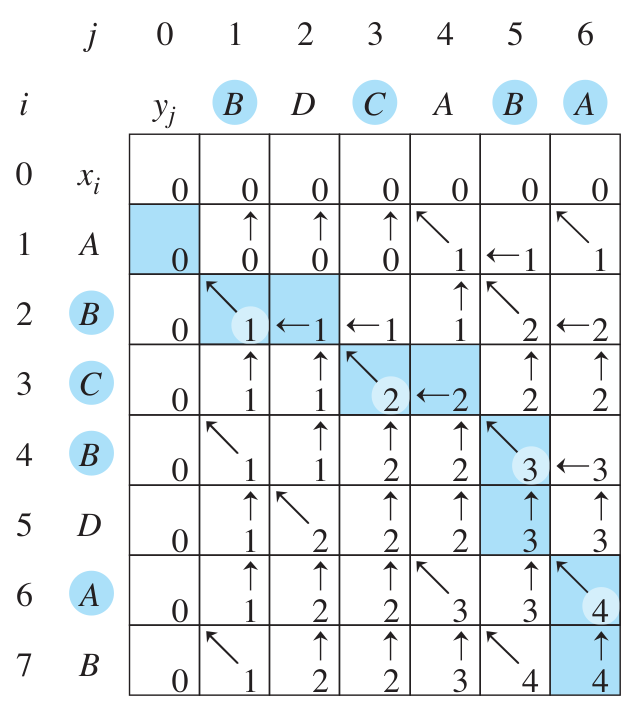
\includegraphics[width=0.4\textwidth]{figs/chap04/lcs-example}
\end{figure}
\end{itemize}
\end{frame}


\begin{frame}{‌طولانی‌ترین زیر رشته مشترک}
\begin{itemize}\itemr
\item[-]
\begin{algorithm}[H]\alglr
  \caption{Print Longest Common Subsequence} 
  \begin{algorithmic}[1]
   \Func{Print-LCS}{b, X, i, j}
		\If{i == 0 or j ==0}
				\State \Return \LeftComment{the longest common subsequence has length 0}
		\EndIf
		\If{b[i, j] == "$\nwarrow$"}
			\State Print-LCS(b, X, i-1, j-1)
			\State print X[i] \LeftComment{same as Y[j]}
		\ElsIf{b[i, j] = "$\uparrow$"}
			\State Print-LCS(b, X, i-1, j)
		\Else{\State Print-LCS(b, X, i, j-1)}
		\EndIf
  \end{algorithmic}
  \label{alg:merge}
\end{algorithm}  
\end{itemize}
\end{frame}




\begin{frame}{‌طولانی‌ترین زیر رشته مشترک}
\begin{itemize}\itemr
\item[-]
پس از طراحی یک الگوریتم معمولاً به دنبال روش‌هایی برای بهبود در زمان اجرا و میزان حافظه می‌گردیم.
\item[-]
در الگوریتم طولانی‌ترین زیر دنبالهٔ مشترک به طور مثال می توانیم جدول b را حذف کنیم و اطلاعات لازم برای ساختن بلندترین زیر دنبالهٔ مشترک را از جدول c به دست آوریم.
\item[-]
هریک از درایه‌های
\m{c[i,j]}
از طریق یکی از سه درایهٔ
\m{c[i-1,j-1]}
،
\m{c[i-1,j]}
،
\m{c[i,j-1]}
محاسبه شده است که در زمان ثابت می‌توانیم بدون جدول b به دست آوریم درایه
\m{c[i,j]}
چگونه محاسبه شده است.
\item[-]
بنابراین طولانی‌ترین زیردنبالهٔ مشترک را می‌توانیم همچنان در زمان
\ath{m+n}
بسازیم و جدول b را حذف کرده و از حافظهٔ مورد نیاز به میزان
mn
بکاهیم.
\end{itemize}
\end{frame}

\begin{frame}{‌درخت جستجوی دودویی بهینه}
\begin{itemize}\itemr
\item[-]
فرض کنید می‌خواهیم برنامه‌ای طراحی کنیم که متون انگلیسی را به فارسی ترجمه کند. به ازای هر کلمهٔ انگلیسی در یک متن باید با استفاده از یک فرهنگ لغت، معادل فارسی آن را بیابیم. برای یک جستجوی بهینه می‌توانیم یک درخت جستجوی دودویی با n رأس بسازیم که هر رأس آن یک کلمهٔ انگلیسی و معادل فارسی آن را شامل شود.
\item[-]
اگر از یک درخت جستجوی دودویی متوازن
\fn{1}{balanced binary search tree}
%مانند درخت قرمز-سیاه
%\fn{2}{red-black tree}
استفاده کنیم، می‌توانیم جستجوی هر کلمه را در یک درخت با n کلمه در زمان
\m{O(\lg n)}
انجام دهیم.
\end{itemize}
\end{frame}

\begin{frame}{‌درخت جستجوی دودویی بهینه}
\begin{itemize}\itemr
\item[-]
اما کلمات مختلف تعداد تکرارهای مختلف دارند. برای مثال کلمات a یا the در انگلیسی بسیار پر تکرارند و بهتر است این کلمات در درخت جستجو به ریشه نزدیک‌تر باشند و برخی از اسامی خاص بسیار کم تکرارند و بهتر است که فاصلهٔ آنها از ریشه بیشتر باشد.
\item[-]
با استفاده از درخت جستجوی دودویی بهینه
\fn{1}{optimal binary search tree}
می‌توان کلمات را به گونه‌ای ذخیره و بازیابی کرد که کلمات با احتمال وقوع بیشتر نزدیک‌تر به ریشه قرار بگیرند.
\end{itemize}
\end{frame}


\begin{frame}{‌درخت جستجوی دودویی بهینه}
\begin{itemize}\itemr
\item[-]
دنبالهٔ
\m{K = \langle k_1, k_2, \cdots , k_n \rangle}
با n کلید را در نظر بگیرید به طوری‌که
\m{k_1 < k_2 < \cdots < k_n} .
\item[-]
می‌خواهیم یک درخت جستجوی دودویی بهینه حاوی این کلیدها بسازیم.
\item[-]
به ازای هر یک از کلیدهای
\m{k_i}
، یک احتمال وقوع
\m{p_i}
نیز داده شده است.
\item[-]
از آنجایی که برخی از کلیدها در درخت جستجو وجود ندارد‌ (برای مثال کلماتی در کاربرد ترجمه در انگلیسی وجود دارند که معادل فارسی ندارند) ، تعداد
\m{n+1}
کلید بی‌استفاده
\m{d_0, d_1, d_2, \cdots, d_n}
نیز داریم که نماینده این کلیدها هستند. در واقع
\m{d_0}
نمایندهٔ همهٔ کلیدهایی است که از
\m{k_1}
کوچکترند و
\m{d_n}
نمایندهٔ همهٔ کلیدهایی است که از
\m{k_n}
بزرگ‌ترند و همچنین به ازای
\m{i = 1,2, \cdots, n-1}
، کلید
\m{d_i}
نمایندهٔ همهٔ مقادیری است که بین
\m{k_i}
و
\m{k_{i+1}}
قرار دارند. همچنین به ازای هر کلید
\m{d_i}
یک احتمال وقوع
\m{q_i}
داریم.
\end{itemize}
\end{frame}


\begin{frame}{‌درخت جستجوی دودویی بهینه}
\begin{itemize}\itemr
\item[-]
در شکل زیر دو درخت جستجوی دودویی بهینه را با تعداد ۵ کلید مشاهده می‌کنیم.
\begin{figure}
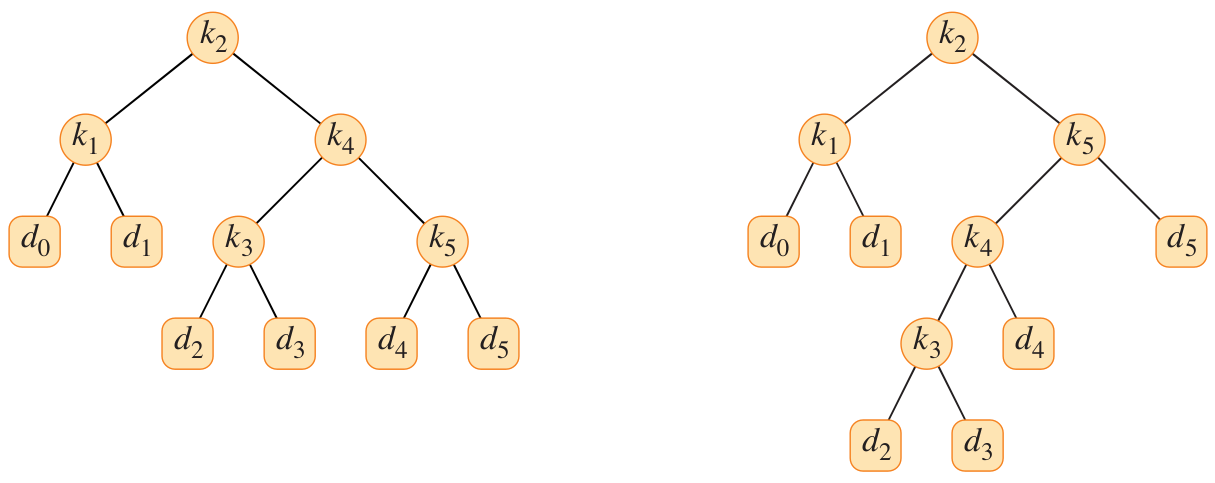
\includegraphics[width=0.9\textwidth]{figs/chap04/optimal-tree}
\end{figure}
\end{itemize}
\end{frame}


\begin{frame}{‌درخت جستجوی دودویی بهینه}
\begin{itemize}\itemr
\item[-]
هر یک از کلیدهای
\m{k_i}
یک رأس میانی است و هر یک از کلیدهای بی‌استفادهٔ
\m{d_i}
یک برگ در درخت جستجوی بهینه است.
\item[-]
از آنجایی که هر جستجو یا موفق است (که منجر به پیدا کردن یک کلید
\m{k_i}
می‌شود) و یا ناموفق (که منجر به رسیدن به کلید بی‌استفادهٔ
\m{d_i}
است)، بنابراین داریم :
\begin{align*}
\m{\sum_{i=1}^n p_i + \sum_{i=0}^n q_i = 1}
\end{align*}
\end{itemize}
\end{frame}


\begin{frame}{‌درخت جستجوی دودویی بهینه}
\begin{itemize}\itemr
\item[-]
با اطلاع داشتن از احتمال وقوع هر یک از کلید‌ها، می‌توانیم هزینه جستجو در یک درخت جستجو را پیدا کنیم.
\item[-]
فرض کنید هزینهٔ جستجوی یک کلید در درخت به ازای هر بار جستجو برابر با تعداد رئوس بررسی شده برای رسیدن به آن کلید باشد. بنابراین هزینهٔ جستجوی یک کلید در یک جستجو برابر خواهد بود با عمق
\fn{1}{depth}
رأس مربوط به آن کلید به علاوهٔ یک. ریشه در عمق صفر قرار دارد، بنابراین هزینهٔ یافتن کلید مربوط به ریشه در یک جستجو برابر است با یک.
\item[-]
برای یافتن هزینهٔ جستجوی یک کلید در یک متن، باید هزینهٔ یک بار جستجو را در احتمال وقوع آن کلید ضرب کنیم.
\item[-]
نهایتا برای یافتن هزینهٔ جستجوی یک درخت باید هزینهٔ جستجوی همهٔ کلیدها را با هم جمع کنیم.
\end{itemize}
\end{frame}

\newcommand{\depth}{\text{depth}}

\begin{frame}{‌درخت جستجوی دودویی بهینه}
\begin{itemize}\itemr
\item[-]
بنابراین هزینهٔ جستجو در درخت T برابر است با :
\begin{align*}
\m{E [\txtlr{search~cost~in}~T]} & \m{~= \sum_{i=1}^n (\depth_T (k_i)+1) \cdot p_i + \sum_{i=0}^n (\depth_T (d_i)+1) \cdot q_i}\\
& \m{~= 1 + \sum_{i=1}^n \depth_T (k_i) \cdot p_i + \sum_{i=0}^n \depth_T (d_i) \cdot q_i}
\end{align*}
\item[-]
در اینجا
\m{\depth_T}
تابعی است که عمق یک کلید را در درخت T نشان می‌دهد.
\end{itemize}
\end{frame}


\begin{frame}{‌درخت جستجوی دودویی بهینه}
\begin{itemize}\itemr
\item[-]
در شکل زیر هزینهٔ جستجو برای دو درخت جستجو محاسبه شده است.
\begin{figure}
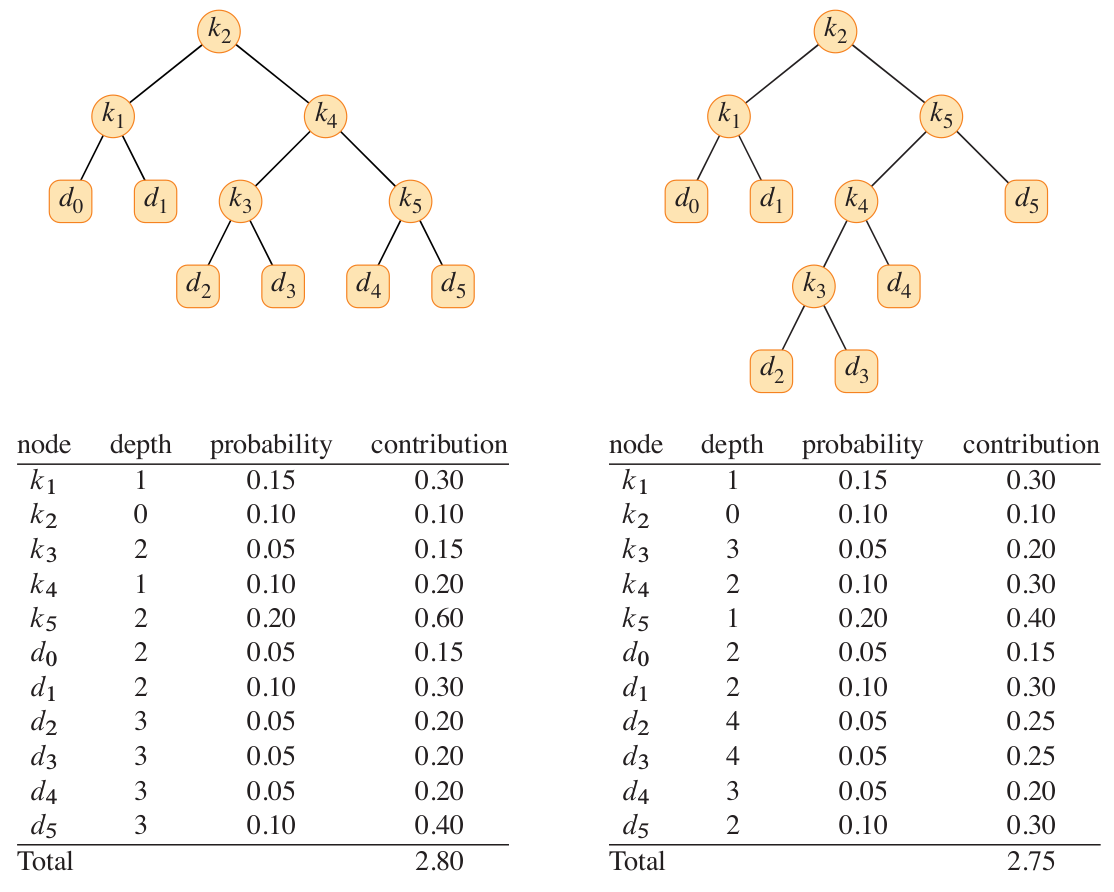
\includegraphics[width=0.6\textwidth]{figs/chap04/tree-cost}
\end{figure}
\end{itemize}
\end{frame}


\begin{frame}{‌درخت جستجوی دودویی بهینه}
\begin{itemize}\itemr
\item[-]
حال به ازای تعدادی کلید به همراه احتمال وقوع آنها، می‌خواهیم یک درخت جستجوی دودویی بیابیم که هزینهٔ جستجو در آن حداقل است.
\item[-]
به این درخت، درخت جستجوی دودویی بهینه
\fn{1}{optimal binary search tree}
گفته می‌شود.
\end{itemize}
\end{frame}


\begin{frame}{‌درخت جستجوی دودویی بهینه}
\begin{itemize}\itemr
\item[-]
در شکل زیر دو درخت جستجوی دودویی نشان داده شده‌اند. هزینهٔ جستجو در درخت سمت چپ
\m{2.80}
و در درخت سمت راست برابر با
\m{2.75}
است. درخت سمت راست یک درخت جستجوی بهینه است. در اینجا می‌توانیم ببینیم درخت جستجوی دودویی بهینه، الزاماً درختی نیست که عمق آن کمتر باشد.
\begin{figure}
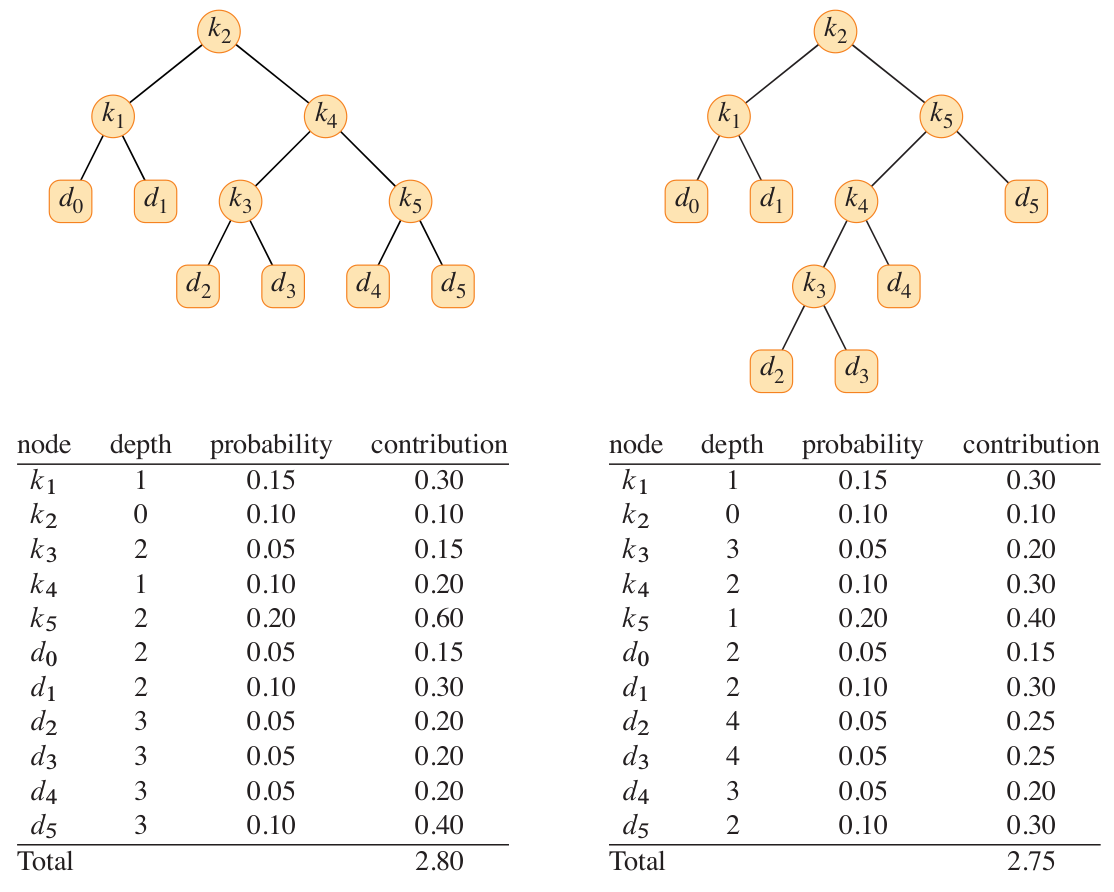
\includegraphics[width=0.5\textwidth]{figs/chap04/tree-cost}
\end{figure}
\end{itemize}
\end{frame}


\begin{frame}{‌درخت جستجوی دودویی بهینه}
\begin{itemize}\itemr
\item[-]
همچنین درخت جستجوی دودویی بهینه الزاماً درختی نیست که همهٔ کلیدها با احتمال وقوع بیشتر در ریشهٔ آن باشند. برای مثال کلید
\m{k_5}
بیشترین احتمال وقوع را دارد، اما ریشهٔ درخت جستجو
\m{k_2}
است.
\end{itemize}
\end{frame}


\begin{frame}{‌درخت جستجوی دودویی بهینه}
\begin{itemize}\itemr
\item[-]
همانند مسئله ضرب زنجیره‌ای ماتریس‌ها، با استفاده از جستجوی کامل برای بررسی همهٔ درخت‌های جستجو نمی‌توانیم در زمان چندجمله‌ای درخت جستجوی دودویی بهینه را به دست آوریم. تعداد همهٔ
 درخت‌های جستجوی دودویی از مرتبهٔ نمایی است، بنابراین بررسی همهٔ درخت‌های جستجو ممکن نیست.
\item[-]
می‌خواهیم این مسئله را با استفاده از برنامه‌ریزی پویا حل کنیم.
\end{itemize}
\end{frame}


\begin{frame}{‌درخت جستجوی دودویی بهینه}
\begin{itemize}\itemr
\item[-]
گام اول : ساختار یک درخت جستجوی دودویی بهینه
\item[-]
برای بررسی ساختار و مشخص کردن ویژگی‌های یک درخت بهینه، ابتدا ساختار درخت و زیردرخت‌های آن را بررسی می‌کنیم.
در واقع باید اثبات کنیم این مسئله دارای زیرساختار بهینه است، بدین معنی که جواب زیرمسئله‌ها را می‌توان از جواب مسئله استخراج کرد.
\item[-]
اگر یک درخت جستجوی دودویی بهینه
\m{T}
داشته باشیم، زیر درخت
\m{T'}
%شامل کلیدهای
%\m{k_i, \cdots, k_j}
%و کلیدهای
%\m{d_{i-1}, \cdots, d_j}
نیز باید بهینه باشد. اگر یک زیر درخت
\m{T''}
وجود داشت که هزینهٔ آن کمتر از
\m{T'}
بود، می‌توانستیم
\m{T'}
را با
\m{T''}
جایگزین کنیم و یک درخت با هزینه کمتر به جای
\m{T}
بیابیم که با فرض بهینه بودن
\m{T}
در تناقض است.
\item[-]
حال می‌خواهیم مسئله را با استفاده از جواب زیر مسئله‌های بهینهٔ آن حل کنیم.
\end{itemize}
\end{frame}


\begin{frame}{‌درخت جستجوی دودویی بهینه}
\begin{itemize}\itemr
\item[-]
یک زیردرخت دلخواه را در نظر بگیرید. این زیردرخت شامل کلیدهای
\m{k_i, \cdots, k_j}
است
که برگ‌های آن را کلیدهای
\m{d_{i-1}, \cdots, d_j}
تشکیل می‌دهند، به طوری‌که
\m{1 \leqslant i \leqslant j \leqslant n} .
\item[-]
به ازای کلیدهای
\m{k_i, \cdots, k_j}
، یکی از این کلیدها، برای مثال کلید
\m{k_r}
به طوری‌که
\m{i \leqslant r \leqslant j}
، ریشهٔ زیردرخت بهینه برای این کلیدهاست.
\item[-]
زیردرخت سمت چپ ریشهٔ
\m{k_r}
شامل کلیدهای
\m{k_i, \cdots, k_{r-1}}
و کلیدهای برگ
\m{d_{i-1}, \cdots, d_{r-1}}
است و زیردرخت سمت راست شامل کلیدهای
\m{k_{r+1}, \cdots, k_j}
و کلیدهای برگ
\m{d_r, \cdots, d_j}
است.
\item[-]
فرض کنید در یک زیردرخت با کلیدهای
\m{k_i, \cdots, k_j}
، کلید
\m{k_i}
را به عنوان ریشه انتخاب کنیم. 
%بنابراین زیردرخت سمت چپ این زیردرخت هیچ رأسی را شامل نمی‌شود. اگر برگ‌ها را نیز در نظر بگیریم، 
زیردرخت سمت چپ این زیردرخت یک برگ با کلید
\m{d_{i-1}}
است.
\item[-]
به طور مشابه، اگر
\m{k_j}
را به عنوان ریشه در نظر بگیریم زیر درخت سمت راست این زیر درخت شامل یک برگ با کلید
\m{d_j}
است.
\end{itemize}
\end{frame}


\begin{frame}{‌درخت جستجوی دودویی بهینه}
\begin{itemize}\itemr
\item[-]
گام دوم : راه حل بازگشتی
\item[-]
حال برای تعریف راه ‌حل بهینه به صورت بازگشتی، زیر درختی شامل کلیدهای
\m{k_i, \cdots, k_j}
را در نظر بگیرید به طوری‌که
\m{i \geqslant 1}
،
\m{j \leqslant n}
و
\m{j \geqslant i-1}
. وقتی
\m{j = i - 1}
باشد، تنها کلید برگ
\m{d_{i-1}}
را خواهیم داشت.
\item[-]
فرض کنید
\m{e[i,j]}
هزینهٔ جستجوی یک درخت جستجوی بهینه با کلیدهای
\m{k_i, \cdots, k_j}
باشد. هدف محاسبهٔ هزینه جستجو برای همهٔ کلیدهاست که برابر با مقدار
\m{e[1,n]}
می‌باشد.
\item[-]
اگر
\m{j = i - 1}
باشد، آنگاه مسئله تنها شامل یک کلید
\m{d_{i-1}}
می‌شود. در اینصورت هزینهٔ جستجو برابراست با
\m{e[i,i-1] = q_{i-1}}.
\item[-]
وقتی
\m{j \geqslant i}
باشد، باید ریشهٔ
\m{k_r}
را از بین کلیدهای
\m{k_i, \cdots, k_j}
انتخاب کنیم و یک درخت جستجوی بهینه با کلیدهای
\m{k_i, \cdots, k_{r-1}}
به عنوان زیردرخت سمت چپ ریشهٔ
\m{k_r}
و یک درخت جستجوی بهینه با کلیدهای
\m{k_{r+1}, \cdots, k_j}
به عنوان زیردرخت سمت راست ریشهٔ
\m{k_r}
بسازیم.
\end{itemize}
\end{frame}


\begin{frame}{‌درخت جستجوی دودویی بهینه}
\begin{itemize}\itemr
\item[-]
وقتی یک زیردرخت بهینه 
\m{T'}
 به عنوان زیردرخت یک رأس قرار می‌گیرد و درخت
\m{T}
را تشکیل می‌دهد،
 درواقع عمق هر یک از رأس‌های 
\m{T'}
در درخت
\m{T}
  یک واحد افزوده می‌شود. در اینصورت هزینهٔ جستجو برای رئوس زیردرخت
\m{T'}
در درخت
\m{T}
   به میزان مجموع احتمال رئوس 
\m{T'}
    افزایش می‌یابد.
\end{itemize}
\end{frame}

\begin{frame}{‌درخت جستجوی دودویی بهینه}
\begin{itemize}\itemr
\item[-]
برای مثال فرض کنید درخت
\m{T'}
 با کلید‌های
\m{k_1,k_2,k_3}
را تشکیل داده باشیم. هزینه جستجوی این درخت (بدون در نظر گرفتن کلیدهای بی‌استفاده) برابر است با
\m{E[T'] = \sum_{i=1}^3 (\depth_{T'}(k_i)+1) \cdot p_{i}  } .
\item[-]
اگر زیردرخت 
\m{T'}
در درخت 
\m{T}
قرار بگیرد به طوری که ریشه درخت 
\m{T}
کلید
\m{k_4}
و
\m{T'}
زیردرخت سمت چپ در درخت 
\m{T}
باشد، آنگاه خواهیم داشت:
\begin{align*}
\m{E[T]} =& \m{~p_4 + \Big(\sum_{i=1}^3 (\depth_{T}(k_i)+1 ) \cdot p_{i} \Big)} \\
=& \m{~p_4 + \Big( \sum_{i=1}^3 (\depth_{T'}(k_i)+2) \cdot p_{i} \Big) } \\
=& \m{~p_4 + E[T'] + \Big( \sum_{i=1}^3 p_{i} \Big) }
\end{align*}
\end{itemize}
\end{frame}

\begin{frame}{‌درخت جستجوی دودویی بهینه}
\begin{itemize}\itemr
\item[-]
برای یک زیردرخت با کلیدهای
\m{k_i, \cdots, k_j}
مجموع  احتمال‌ها برابر است با :
\begin{align*}
\m{w(i,j) = \sum_{l=i}^j p_l + \sum_{l=i-1}^j q_l}
\end{align*}
\item[-]
بنابراین اگر
\m{k_r}
ریشهٔ یک زیردرخت بهینه با کلیدهای
\m{k_i, \cdots, k_j}
باشد، خواهیم داشت :
\begin{align*}
\m{e[i,j] = p_r + (e[i,r-1] + w(i,r-1)) + (e[r+1,j] + w(r+1,j))}
\end{align*}
\end{itemize}
\end{frame}

\begin{frame}{‌درخت جستجوی دودویی بهینه}
\begin{itemize}\itemr
\item[-]
 از آنجایی که مجموع احتمال وقوع همهٔ رئوس در یک درخت برابر است با مجموع احتمال‌های وقوع رئوس زیردرخت چپ به علاوهٔ احتمال وقوع ریشه به علاوهٔ احتمال‌های وقوع رئوس زیردرخت راست، بنابراین رابطه زیر برقرار است :
\begin{align*}
\m{w(i,j) = w(i,r-1) + p_r + w(r+1,j)}
\end{align*}
\item[-]
بنابراین می‌توانیم رابطه بازگشتی برای محاسبه هزینهٔ جستجو در درخت بهینه را به صورت زیر بازنویسی کنیم :
\begin{align*}
\m{e[i,j] = e[i,r-1] + e[r+1,j] + w(i,j)}
\end{align*}
\end{itemize}
\end{frame}


\begin{frame}{‌درخت جستجوی دودویی بهینه}
\begin{itemize}\itemr
\item[-]
در اینجا فرض کردیم که می‌دانیم کدام رأس به عنوان رأس ریشهٔ
\m{k_r}
انتخاب می‌شود.
\item[-]
از آنجایی که هدف این است که ریشه‌ای را انتخاب کنیم که مقدار هزینه جستجو را کاهش دهد، بنابراین رابطهٔ بازگشتی برای محاسبهٔ هزینه جستجو در درخت بهینه را به صورت زیر می‌نویسیم.
\begin{align*}
\m{e[i,j]} = \left\{ \begin{array}{lr}
					\m{q_{i-1}} & \m{j=i-1}~~\text{اگر}\\
					\m{\min\{e[i,r-1] + e[r+1,j] + w(i,j) : i \leqslant r \leqslant j \}} & \m{i \leqslant j}~~ \text{اگر}
					\end{array}\right.
\end{align*}
\item[-]
بنابراین رابطه‌ای برای جدول
\m{e[i,j]}
جهت استفاده در یک الگوریتم برنامه‌ریزی پویا به صورت بازگشتی محاسبه کردیم.
\end{itemize}
\end{frame}


\begin{frame}{‌درخت جستجوی دودویی بهینه}
\begin{itemize}\itemr
\item[-]
جدول
\m{e[i,j]}
 تنها میزان هزینه جستجوی بهینه را نگهداری می‌کند.
\item[-]
 به یک جدول دیگر نیاز داریم برای اینکه بتوانیم ساختار درخت را نیز نگهداری کنیم تا در نهایت بتوانیم درخت جستجو بهینه را بازسازی کنیم.
\item[-]
این اطلاعات را در جدول
\m{root[i,j]}
نگهداری می‌کنیم. درواقع مقدار
\m{root[i,j]}
به ازای
\m{1 \leqslant i \leqslant j \leqslant n}
برابراست با اندیس r برای کلید
\m{k_r}
که ریشهٔ درخت جستجوی بهینه‌ای است که برای کلیدهای
\m{k_i, \cdots, k_j}
یافته می‌شود.
\end{itemize}
\end{frame}


\begin{frame}{‌درخت جستجوی دودویی بهینه}
\begin{itemize}\itemr
\item[-]
گام سوم : محاسبهٔ هزینهٔ جستجو در یک درخت جستجوی دودویی بهینه
\item[-]
حال با استفاده از روش برنامه‌ریزی پویا می‌توانیم مقادیر
\m{e[i,j]}
را به ترتیب از پایین به بالا محاسبه می‌کنیم. بنابراین کل جدول را به ازای
\m{e[1:n+1,0:n]}
مقداردهی می‌کنیم.
\item[-]
اندیس اول از 
\m{1}
 شروع شده و با
\m{n+1}
خاتمه می‌یابد، زیرا برای داشتن یک زیردرخت شامل تنها کلید
\m{d_n}
نیاز داریم
\m{e[n+1,n]}
را محاسبه کنیم. اندیس دوم باید از صفر شروع شود، زیرا برای داشتن یک زیردرخت تنها با کلید
\m{d_0}
، باید مقدار
\m{e[1,0]}
را محاسبه کنیم.
\item[-]
همهٔ مقادیر
\m{e[i,j]}
به ازای
\m{j \geqslant i-1}
باید محاسبه شوند. جدول
\m{root[i,j]}
ریشهٔ زیردرخت‌ها را با کلیدهای
\m{k_i, \cdots, k_j}
ذخیره می‌کند، به طوری‌که
\m{1 \leqslant i \leqslant j \leqslant n}.
\end{itemize}
\end{frame}


\begin{frame}{‌درخت جستجوی دودویی بهینه}
\begin{itemize}\itemr
\item[-]
همچنین می‌توانیم از یک جدول دیگر بهره بگیریم تا محاسبات را سریع‌تر انجام دهیم.
\item[-]
به جای محاسبه
\m{w(i,j)}
برای هر یک از درایه‌های
\m{e[i,j]}
%که به زمان
%\ath{j-i}
%نیاز دارد، 
جدول
\m{w[1:n+1,0:n]}
را محاسبه می‌کنیم. در حالت پایه، مقدار
\m{w[i,i-1] = q_{i-1}}
به ازای
\m{1 \leqslant i \leqslant n+1}
\item[-]
به ازای
\m{j \geqslant i}
درایه‌های جدول w را به صورت زیر محاسبه می‌کنیم.
\begin{align*}
\m{w[i,j] = w[i,j-1] + p_j + q_j}
\end{align*}
\item[-]
بنابراین می‌توانیم
\ath{n^2}
مقدار
\m{w[i,j]}
را هرکدام در زمان
\ath{1}
محاسبه کنیم.
% و مقادیر ذخیره شده در جدول را در زمان اجرا بازیابی کنیم.
\end{itemize}
\end{frame}


\begin{frame}{‌درخت جستجوی دودویی بهینه}
\begin{itemize}\itemr
\item[-]
الگوریتم زیر مسئلهٔ درخت جستجوی دودویی بهینه را به روش برنامه‌ریزی پویا حل می‌کند.
\begin{algorithm}[H]\alglr
  \caption{Optimal-BST} 
  \begin{algorithmic}[1]
   \Func{Optimal-BST}{p, q, n}
    \State let e[1:n+1 , 0:n], w[1:n+1 , 0:n], and root[1:n , 1:n] be new tables
    \For{i = 1 \To n + 1} \LeftComment{base cases} 
      \State e[i,i-1] = q[i-1]
      \State w[i,i-1] = q[i-1]
    \EndFor                        
  \end{algorithmic}
  \label{alg:merge}
\end{algorithm}
\end{itemize}
\end{frame}


\begin{frame}{‌درخت جستجوی دودویی بهینه}
\begin{itemize}\itemr
\item[-]
\begin{algorithm}[H]\alglr
  \caption{Optimal-BST} 
  \begin{algorithmic}[1]
  \setcounter{ALG@line}{4}
   \Func{Optimal-BST}{p, q, n}
    \For{t = 1 \To n}
    	\For{i = 1 \To n - t + 1}
    		\State j = i + t - 1
    		\State e[i,j] = $\infty$
    		\State w[i,j] = w[i,j-1] + p[j] + q[j]
    		 \For{r = i \To j} \LeftComment{try all possible roots r}
    		 		\State t = e[i,r-1] + e[r+1,j] + w[i,j] 
    		 		\If{t < e[i,j]} \LeftComment{new minimum?}
    		 				\State e[i,j] = t
    		 				\State root[i,j] = r
    		 		\EndIf
    		 \EndFor
    	\EndFor
    \EndFor
   \State \Return e and root                         
  \end{algorithmic}
  \label{alg:merge}
\end{algorithm}
\end{itemize}
\end{frame}


\begin{frame}{‌درخت جستجوی دودویی بهینه}
\begin{itemize}\itemr
\item[-]
الگوریتم درخت جستجوی دودویی بهینه محاسبات را در زمان
\ath{n^3}
انجام می‌دهد و به یک جدول با اندازهٔ
\ath{n^2}
نیاز دارد.
\end{itemize}
\end{frame}


\begin{frame}{‌درخت جستجوی دودویی بهینه}
\begin{itemize}\itemr
\item[-]
در شکل زیر، جدول‌های
\m{e[i,j]}
،
\m{w[i,j]}
و
\m{root[i,j]}
با استفاده از الگوریتم برنامه‌ریزی پویا برای جستجوی دودویی بهینه برای کلید‌های تعیین شده زیر، محاسبه شده‌اند.
\begin{figure}
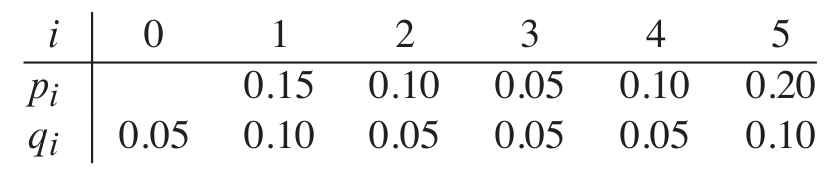
\includegraphics[width=0.5\textwidth]{figs/chap04/key-prob-example}
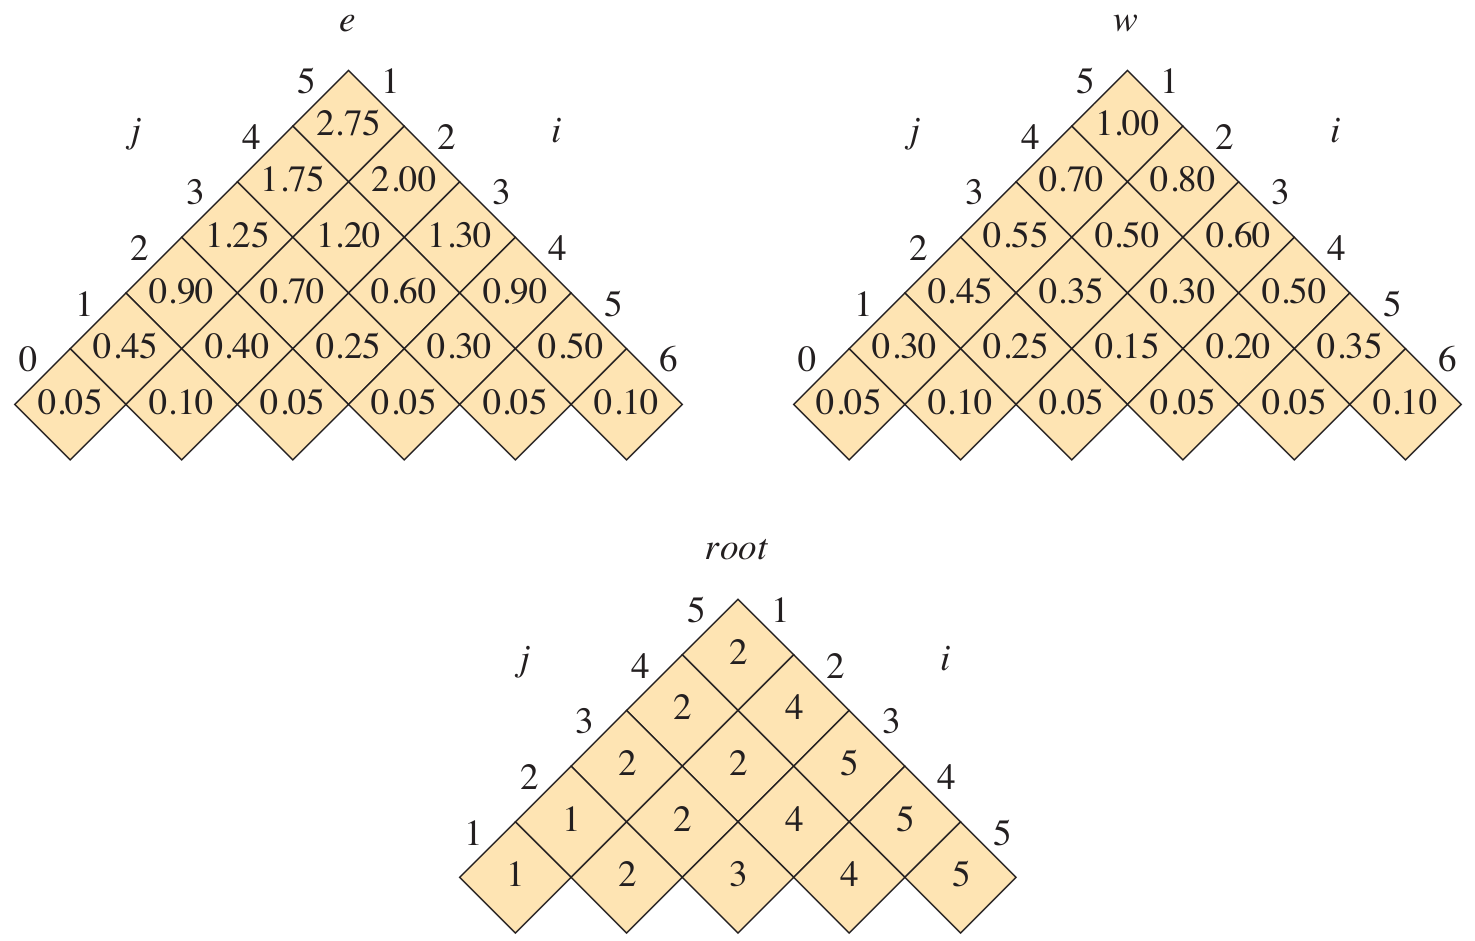
\includegraphics[width=0.5\textwidth]{figs/chap04/bst-example}
\end{figure}
\end{itemize}
\end{frame}
\newcommand{\itm}{\text{item}}
\begin{frame}{‌کوله‌پشتی ۱-۰}
\begin{itemize}\itemr
\item[-]
یک دزد با یک کوله‌پشتی به یک فروشگاه دستبرد می‌زند. وزنی که کوله‌پشتی او می‌تواند تحمل کند
\m{W}
است. در این فروشگاه تعداد
\m{n}
کالا وجود دارد. هر کالای
\m{\itm_i}
دارای وزن
\m{w_i}
و ارزش
\m{v_i}
است. دزد می‌خواهد از میان این کالاها تعدادی را انتخاب کرده در کوله‌پشتی خود قرار دهد به طوری‌که مجموع وزن کالاهای انتخاب شده از ظرفیت کوله‌پشتی یعنی
\m{W}
بیشتر نباشد و مجموع ارزش کالاهای دزدیده شده حداکثر باشد.
\item[-]
بنابراین دزد می‌خواهد از مجموعهٔ
\m{S = \{\itm_1 ,\itm_2 , \cdots ,\itm_n \} }
یک زیر مجموعه
\m{A}
را انتخاب کند به طور
\m{\sum_{\itm_i \in A} v_i}
بیشترین مقدار ممکن باشد و
\m{(\sum_{\itm_i \in A} w_i) \leqslant W}
باشد.
\item[-]
تعداد همهٔ حالت‌های ممکن تعداد همهٔ زیر مجموعه‌های
\m{S}
است که برابر است با
\m{2^n}
جایی که
\m{n}
تعداد کالاهاست.
\item[-]
در این مسئله دزد یا می‌تواند یک کالا را بردارد یا بگذارد و امکان شکستن کالاها به دو قسمت وجود ندارد. به همین دلیل به آن مسئله کوله پشتی ۱-۰
\fn{1}{\m{0}-\m{1} knapsack}
گفته می‌شود. در مسئلهٔ کوله‌پشتی کسری
\fn{2}{fractional knapsack}
دزد می‌تواند یک کالا را به دو قسمت تقسیم کرده، یک قسمت را در کوله‌پشتی قرار دهد و قسمت دیگر را در فروشگاه بگذارد.
\end{itemize}
\end{frame}


\begin{frame}{‌کوله‌پشتی ۱-۰}
\begin{itemize}\itemr
\item[-]
در گام اول باید اثبات کنیم این مسئله دارای زیر ساختار بهینه است یا به عبارت دیگر قانون بهینگی
\fn{1}{principle of optimality}
برای آن صادق است.
\item[-]
فرض کنید
\m{A}
زیر مجموعه بهینه از
\m{n}
کالا باشد. دو حالت وجود دارد : یا
\m{A}
شامل
\m{\itm_n}
می‌شود یا خیر.
\item[-]
اگر
\m{A}
کالای
\m{\itm_n}
را شامل نشود،
\m{A}
یک زیر مجموعه بهینه برای
\m{n-1}
کالا نیز هست.
\item[-]
اگر
\m{A}
کالای
\m{\itm_n}
را شامل شود، آنگاه مجموع ارزش‌های کالاهای
\m{A}
برابر است با
\m{v_n}
به علاوه بیشترین ارزش ممکن که از
\m{n-1}
کالا برای یک کوله‌پشتی با ظرفیت
\m{W-w_n}
به دست آمده است. این گزاره‌ها را می‌توانیم با برهان خلف اثبات کنیم.
\end{itemize}
\end{frame}


\begin{frame}{‌کوله‌پشتی ۱-۰}
\begin{itemize}\itemr
\item[-]
در گام دوم باید یک رابطه بازگشتی برای محاسبه جواب مسئله براساس جواب زیر مسئله‌ها بنویسیم.
\item[-]
%اگر
%\m{i > 0}
%و
%\m{w > 0}
%باشد آنگاه
فرض کنید
\m{P[i][w]}
بیشترین ارزش به دست آمده از
\m{i}
کالای اول است وقتی که ظرفیت کوله‌پشتی
\m{w}
باشد.
\item[-]
می‌توانیم یک رابطه بازگشتی به صورت زیر برای محاسبه
\m{P[i][w]}
بنویسیم.
\begin{align*}
\m{P[i][w]} = \left\{\begin{array}{lr}
          \m{\max (P[i-1][w] , v_i + P[i-1][w-w_i])}&\m{w_i \leqslant w}~\text{اگر}\\
          \m{P[i-1][w]}&\m{w_i > w}~\text{اگر}
\end{array}\right.
\end{align*}
\item[-]
در این مسئله به دنبال
\m{P[n][W]}
می‌گردیم.
\end{itemize}
\end{frame}


\begin{frame}{‌کوله‌پشتی ۱-۰}
\begin{itemize}\itemr
\item[-]
می‌توانیم جدولی تشکیل دهیم که هر سطر
\m{i}
در آن نشان دهنده این باشد که فقط از
\m{i}
کالای اول استفاده کرده‌ایم و ستون‌های آن همهٔ وزن‌های ممکن از
\m{0}
تا
\m{W}
باشد.
\item[-]
مقادیر
\m{P[0][w]}
و
\m{P[i][0]}
برابر با صفر هستند.
\item[-]
این جدول دارای
\m{nW}
خانه است پس محاسبه این جدول در زمان
\ath{nW}
امکان‌پذیر است.
\end{itemize}
\end{frame}


\begin{frame}{‌کوله‌پشتی ۱-۰}
\begin{itemize}\itemr
\item[-]
توجه کنید که هیچ رابطه‌ای بین
\m{n}
و
\m{W}
وجود ندارد و این الگوریتم می‌تواند از الگوریتمی که همه حالات را بررسی می‌کند بدتر باشد. برای مثال اگر
\m{W = n!}
باشد الگوریتم برنامه‌ریزی پویا از مرتبه
\m{n!}
است درحالی که بررسی همه حالات در زمان
\ath{2^n}
امکان‌پذیر است.
\item[-]
بنابراین تنها در صورتی از برنامه‌ریزی پویا استفاده می‌کنیم که
\m{nW < 2^n}
باشد.
\item[-]
پیچیدگی زمانی
\ath{nW}
گرچه شبیه به پیچیدگی زمانی چندجمله‌ای است، اما در واقع چندجمله‌ای نیست و مقدار 
\m{W}
می‌تواند یک تابع غیرچندجمله‌ای از ورودی مسئله باشد. این پیچیدگی زمانی را پیچیدگی زمانی شبه‌چندجمله‌ای
\fn{1}{pseudo-polynomial time complexity}
می‌نامیم.
\end{itemize}
\end{frame}

\begin{frame}{‌سریع‌ترین مسیر در جدول}
\begin{itemize}\itemr
\item[-]
جدول
\m{A}
با
\m{m}
سطر و
\m{n}
ستون را در نظر بگیرید به طوری‌که مقدار هرکدام از درایه‌های جدول یک عدد صحیح است.
\item[-]
می‌خواهیم مهره‌ای را با شروع از درایه
\m{(1,1)}
حرکت داده، به درایهٔ
\m{(m,n)}
منتقل کنیم. فرض کنید درایهٔ
\m{(1,1)}
در شمال غرب و درایهٔ
\m{(m,n)}
در جنوب شرق جدول قرار دارد.
\item[-]
وقتی مهره وارد درایهٔ
\m{(i,j)}
می‌شود، باید
\m{A[i,j]}
ثانیه در آن درایه صبر کند و پس از آن به حرکت ادامه دهد.
\item[-]
با فرض اینکه مهره تنها می‌تواند به سمت جنوب یا شرق یا مورب به جنوب شرق حرکت کند، می‌خواهیم کمترین زمان ممکن برای انتقال مهره از درایهٔ
\m{(1,1)}
به
\m{(m,n)}
را محاسبه کنیم.
\end{itemize}
\end{frame}


\begin{frame}{‌سریع‌ترین مسیر در جدول}
\begin{itemize}\itemr
\item[-]
در گام اول بررسی می‌کنیم مسئله دارای زیر ساختار بهینه است یا اصل بهینگی در آن برقرار است.
\item[-]
اگر از درایهٔ
\m{(1,1)}
مهره را حرکت داده در کمترین زمان ممکن به درایهٔ
\m{(i,j)}
برسیم حتما از یکی از سه درایهٔ
\m{(i-1,j)}
یا
\m{(i,j-1)}
یا
\m{(i-1,j-1)}
عبور کرده‌ایم.
\item[-]
در صورتی که از
\m{(i-1,j)}
عبور کرده باشیم الزاما برای حرکت از درایه
\m{(1,1)}
به
\m{(i-1,j)}
کمترین زمان ممکن را صرف کرده‌ایم. این گزاره را می‌توانیم با برهان خلف اثبات کنیم.
\item[-]
به همین ترتیب ممکن است از درایه‌های
\m{(i,j-1)}
یا
\m{(i-1,j-1)}
عبور کرده باشیم که به طور مشابه می‌توانیم اثبات کنیم الزاما در کمترین زمان ممکن به این درایه‌ها رسیده‌ایم.
\end{itemize}
\end{frame}


\begin{frame}{‌سریع‌ترین مسیر در جدول}
\begin{itemize}\itemr
\item[-]
در گام دوم رابطه‌ای برای توصیف جواب مسئله براساس جواب زیر مسئله‌ها به صورت زیر می‌نویسیم.
\begin{align*}
\m{T[i,j]} = \left\{\begin{array}{lr}
          \m{\min(T[i-1,j],T[i,j-1],T[i-1,j-1]) + A[i,j]}&\m{j > 1 , i > 1}~\text{اگر}\\
          \m{T[i-1,1] + A[i,1]}&\m{j = 1 , i > 1}~\text{اگر}\\
          \m{T[1,j-1] + A[1,j]}&\m{i = 1 , j > 1}~\text{اگر}\\
          \m{A[1,1]}&\m{j = 1 , i = 1}~\text{اگر}
\end{array}\right.
\end{align*}
\end{itemize}
\end{frame}


\begin{frame}{‌سریع‌ترین مسیر در جدول}
\begin{itemize}\itemr
\item[-]
سپس جدول
\m{T}
را در زمان
\ath{mn}
تکمیل می‌کنیم و
\m{T[m,n]}
جواب مسئله است.
\end{itemize}
\end{frame}
%%%%%%%%%%%%

%%%%%%%%%%%%
%\section*{References}
%\begin{frame}<0>[noframenumbering]
%\bibliographystyle{apalike}
%\bibliography{docs/bib}
%\end{frame}
%%%%%%%%%%%%

\end{document}
